\documentclass[a4paper, 12pt, twoside]{report}

\usepackage{fontspec}
\usepackage{xunicode}
\usepackage{xltxtra}
\usepackage{xgreek}
\usepackage{csquotes}
\usepackage{hyperref}
\usepackage{placeins}

\raggedbottom
\onecolumn

\usepackage{graphicx, amsfonts, psfrag, fancyhdr, layout, subfigure}
\usepackage{pdflscape}
%\usepackage{lscape}
\usepackage{multirow}
\usepackage{longtable}
\usepackage{array}
%The arydshln package offers you the \hdashline and \cdashline commands which are the dashed counterparts of \hline and \cline, respectively. 
\usepackage{arydshln}

\usepackage[toc,page]{appendix}
\renewcommand{\appendixtocname}{Παραρτήματα}
\renewcommand{\appendixname}{Παράρτημα}
\renewcommand{\appendixpagename}{Παραρτήματα}

\setmainfont[Mapping=tex-text]{GFS Artemisia}

\usepackage[style=numeric, bibstyle=numeric, hyperref=true, backref=true, alldates=terse, indexing=false, backend=bibtex]{biblatex}
\addbibresource{Bibliography.bib}

\usepackage{index}
\usepackage[columns=2]{idxlayout}
\newindex{default}{idx}{ind}{Ευρετήριο}

% Set equal margins on book style
\setlength{\oddsidemargin}{53pt}
\setlength{\evensidemargin}{53pt}
\setlength{\marginparwidth}{57pt}
\setlength{\footskip}{30pt}

\author{Καφετζής Δημήτριος Ανδρέας}
\title{Εναέρια λήψη εικόνας - Πρώτη τεχνική έκθεση : Μελέτη σύστασης/κατασκευής πλήρους συστήματος εναέριας λήψης εικόνας}

\begin{document}
	
	\maketitle
	
	\section*{Περίληψη}
		\paragraph{}{Με την αναφορά αυτή επιχειρείται να αποσαφηνιστεί το ίδιο το σύστημα της εναέριας λήψης εικόνας. Παρουσιάζονται τα επί μέρους τμήματα και προτείνονται λύσεις.
		}
		
	\addcontentsline{toc}{chapter}{Περιεχόμενα}
	\tableofcontents

	\newpage
	\phantomsection
	\addcontentsline{toc}{chapter}{Κατάλογος Σχημάτων}
	\listoffigures

	\newpage
	\phantomsection
	\addcontentsline{toc}{chapter}{Κατάλογος Πινάκων}
	\listoftables
	
% Code for creating empty pages
% No headers on empty pages before new chapter
	\makeatletter
		\def\cleardoublepage{
			\clearpage\if@twoside \ifodd\c@page\else
	    	\hbox{}
	    	\thispagestyle{plain}
	    	\newpage
    		\if@twocolumn\hbox{}\newpage\fi\fi\fi
    	}
	\makeatother \clearpage{\pagestyle{plain}\cleardoublepage}

% Define pagestyle
	\pagestyle{fancy}
	\fancyhf{}
	\renewcommand{\chaptermark}[1]{\markboth{ \emph{#1}}{}}

% Adjustments headers
	\fancyhead[LO]{\emph{Κεφάλαιο \thechapter}}
	\fancyhead[RE]{\leftmark}
	\fancyfoot[LE,RO]{\thepage}
	
	\chapter{Εισαγωγή}
		
		\section{Σκοπός}
			\paragraph{}{Σκοπός μας είναι η σύνθεση και κατασκευή ενός συστήματος εναέριας λήψης φωτογραφιών και βίντεο υψηλής ανάλυσης σε ποικίλες καιρικές συνθήκες. Τα συστήματα αυτά χαρακτηρίζονται ως μη επανδρωμένες εναέριες μηχανές (Uav, Unmanned aerial vehicle)
			}
			
		\section{Γενικές απαιτήσεις}
			\paragraph{}{Η κατασκευή και η λειτουργία του συστήματος θα πρέπει να γίνει λαμβάνοντας υπόψιν τους παρακάτω παραμέτρους :
				\begin{itemize}
					\item Ασφάλεια - εξοπλισμού και περιβάλλοντος
					\item Ευχρηστία – πτήσης και λήψης εικόνας
					\item Λειτουργικότητα – πτήσης και λήψης εικόνας
					\item Ποιότητα – εξοπλισμού, πτήσης και λαμβανόμενης εικόνας
					\item Διάρκεια – πτήσης και λαμβανόμενης εικόνας
Κόστος
				\end{itemize}
			}
			
			\paragraph{Ασφάλεια}{Το σύστημα θα πρέπει να είναι ασφαλές, αφενός για τον εαυτό του με σκοπό την προστασία του εξοπλισμού και την αποφυγή καταπόνησης του και αφετέρου για τους χρήστες και το ευρύτερο περιβάλλον στο οποίο θα λειτουργεί.

 			\paragraph{Ευχρηστία}{Το σύστημα όντας εύχρηστο θα μας απαλλάξει από δυσάρεστες καταστάσεις. Απαιτούμενος σκοπός είναι η πτήση και η λήψη εικόνας να γίνονται όσο το δυνατόν ομαλά και ευχάριστα για τους χειριστές. Η εμπλεκόμενες διαδικασίες θα πρέπει να είναι αυτοματοποιημένες σε μεγάλο βαθμό δίνοντας τη δυνατότητα στους χειριστές να επικεντρωθούν στην ποιότητα του τελικού αποτελέσματος.

 			\paragraph{Λειτουργικότητα}{Θα πρέπει να παρέχονται οι κατάλληλες προϋποθέσεις στους χειριστές του συστήματος για την παραγωγή υψηλής ποιότητας εικόνας και μεγάλου αισθητικού ενδιαφέροντος.

 			\paragraph{Ποιότητα}{Ο παράγοντας αυτός αφορά τόσο τα κατασκευαστικά χαρακτηριστικά του εξοπλισμού, όσο και την ποιότητα της πτήσης και της καταγραφόμενης εικόνας. Ο εξοπλισμός οφείλεται να αντέξει στο χρόνο με εμφάνιση ελαχίστων προβληματικών εξαρτημάτων ή υποσυστημάτων και με διακριτική συντήρηση τους. Επιπλέον, η πτήση αναμένεται να είναι τόσο ομαλή και ανεπηρέαστη από τις διάφορες καιρικές συνθήκες (αέρας, βροχή, χιόνι) ώστε να αποτελεί αιτία για λήψη χαμηλής ποιότητας φωτογραφιών και βίντεο. Αναφορικά με την ίδια την ποιότητα της λαμβανόμενης εικόνας επιθυμείτε να είναι η μέγιστη δυνατή αν όχι υψηλής ανάλυσης (high definition).

 			\paragraph{Διάρκεια}{Το σύστημα θα πρέπει να επιτρέπει την αδιάλειπτη καταγραφή εικόνας για μεγάλο χρονικό διάστημα. Ως ενδεικτικός χρόνος συνεχόμενης πτήσης αναφέρονται τα σαράντα (40) λεπτά, ενώ για το χρόνο καταγραφής οι δύο (2)  με δυόμιση (2 και 1/2) ώρες.

 			\paragraph{Κόστος}{Το κόστος απαιτείται να κυμανθεί στο χαμηλότερο δυνατό επίπεδο. Η σύσταση του συστήματος οφείλεται να γίνει λαμβάνοντας υπόψιν τον υπάρχων εξοπλισμό.
 			
 	\chapter{Τεχνική ανάλυση}
		\section{Εισαγωγή}
			\paragraph{}{Στο κεφάλαιο αυτό θα παρουσιάσουμε τα μέρη από τα οποία θα αποτελείται το σύστημα. Θα καταγραφούν τα χαρακτηριστικά που πρέπει να έχει το κάθε τμήμα του ώστε να πληρούνται οι απαιτήσεις που τέθηκαν στο προηγούμενο κεφάλαιο.
			}
			
			\paragraph{}{Ας ξεκαθαρίσουμε από τι μέρη θα αποτελείται το εν λόγω σύστημα.
			\begin{itemize}
				\item πλατφόρμα πτήσης
				\item πλατφόρμα προσγείωσης
				\item αυτόματος πιλότος
				\item χειροκίνητη πτήση
				\item επίγειος σταθμός ελέγχου πτήσης
				\item πλατφόρμα της μηχανής
				\item αυτόματος πιλότος για την πλατφόρμα της μηχανής
				\item επίγειος σταθμός ελέγχου της πλατφόρμας της μηχανής
				\item μηχανή
				\item σταθμός ελέγχου της μηχανής
				\item εναέριος σταθμός μετάδοσης εικόνας
				\item επίγειος σταθμός λήψης σύγχρονης εικόνας
				\item επίγειος σταθμός καταγραφής της εικόνας
			\end{itemize}
			}
		
		
		\section{Πτητική μηχανή}
		\subsection{Πλατφόρμα πτήσης και προσγείωσης}
			\paragraph{πλατφόρμα πτήσης}{Αναφέρεται στην πτητική συσκευή. Για λόγους ευστάθειας, ασφάλειας, ευχρηστίας, συντήρησης οδηγούμαστε στην επιλογή ενός ηλεκτρικού μέσου και συγκεκριμένα ενός πολυπτέρου. Το πλήθος των κινητήρων δεν έχει αποσαφηνιστεί. Επιλογές αποτελούν τα εξάπτερα και τα οχτάπτερα.
			}
			\paragraph{}{Κάθε πολύπτερο απαρτίζεται από τον σκελετό, τους κινητήρες, τους ελεγκτές των κινητήρων και τους έλικες. Στην αγορά διατίθενται μοντέλα που περιλαμβάνουν όλα αυτά τα υποσυστήματα και μοντέλα που αποτελούνται μόνο από το σκελετό δίνοντας την ευελιξία για την χρήση κινητήρων της επιλογής μας. Για τα τελευταία μοντέλα θα χρειαστεί η συμβουλή και η πιθανότητα η συναρμολόγηση τους από ειδικό πάνω στον
			}
			\paragraph{}{Η πλατφόρμα αυτή μαζί με τη βάση για τη μηχανή αποτελούν τα κυριότερα υποσυστήματα αφού θα καθορίσουν και την επιλογή των υπολοίπων. Στα βασικά χαρακτηριστικά της πτητικής πλατφόρμας πρέπει να περιλαμβάνονται η εύκολη και γρήγορη συναρμολόγηση της, η ανύψωση όσο το δυνατόν μεγαλύτερου φορτίου, η προστασία του περιβάλλοντος της από τους περιστρεφόμενους έλικες. Επιπλέον, η μεγαλύτερη δυνατή παρουσία στον αέρα και αντιμετώπιση διαφορετικών καιρικών συνθηκών αποτελούν σημαντικοί παράγοντες.
			}			
			\paragraph{πλατφόρμα προσγείωσης}{Αναφέρεται στα "πόδια" του συστήματος. Συνήθως αποτελούν ενιαίο τμήμα με την πλατφόρμα πτήσης.
			}
			\paragraph{}{Οι εταιρίες που δραστηριοποιούνται στο χώρο των πολυπτέρων διαθέτουν όλες τους μοντέλα που ικανοποιούν επί το πλείστον τις απαιτήσεις μας. Έχουν ικανοποιητική δύναμη για να ανυψώσουν το βάρος όλου του συστήματος, συναρμολογούνται μέσα σε 5 με 10 λεπτά και μπορούν να συντηρηθούν εύκολα και γρήγορα. Επιπλέον, τα προτεινόμενα συστήματα υποστηρίζονται συνεχώς από τις κατασκευάστριες εταιρίες με αποτέλεσμα να διορθώνονται τυχόν δυσλειτουργίες, να παρουσιάζονται αναβαθμίσεις παρουσιάζονται και να μην υπάρχει έλλειψη ανταλλακτικών.
			}
			\paragraph{}{Από τα απαιτούμενα χαρακτηριστικά κανένα από τα προτεινόμενα μοντέλα δεν διαθέτει σύστημα προστασίας από τους περιστρεφόμενους έλικες. Γενικά η αγορά υπολείπεται στον τομέα αυτό. Έχουν υπάρξει κάποιες προσπάθειες αλλά δεν αποτελούν αξιόπιστη λύση. Η μόνη εν αναμονή λύση προέρχεται από την εταιρία Safeflight Copters\footnote{ιστοσελίδα : \url{http://safeflightcopters.com/}}. Δυστυχώς όμως δεν έχει φτάσει ακόμα στο στάδιο της διάθεσης.
			}
			\paragraph{}{Τέλος, μόνο η εταιρία Droidworx προσφέρει σύστημα προστασίας του εξοπλισμού. Συγκεκριμένα στο πάνω μέρος της πλατφόρμας τοποθετούνται προστατευτικές μπάρες ή προστατευτικό κάλυμμα, το οποίο κάλυμμα προφυλάσσει και από βροχή.
			}
			
		\subsubsection{Εξάπτερα μοντέλα}
			\paragraph{}{Στον πίνακα \ref{πιν.:Μοντέλα εξαπτέρων} παρουσιάζονται τα προτεινόμενα μοντέλα.
			}
			\paragraph{DJI Spreading Wings S800}{Εξάπτερο της εταιρίας DJI που ενσωματώνει και το σύστημα προσγείωσης. Κεντρικό εξάρτημα αποτελεί η κεντρική πλατφόρμα στην οποία ενσωματώνονται τα υπόλοιπα συστήματα. Διαθέτει και ειδικό χώρο για την IMU μονάδα του αυτόματου πιλότου της ίδιας της εταιρίας. Επιπλέον, οι βραχίονες έχουν ενσωματωμένους τα κυκλώματα οδήγησης των κινητήρων και τα απαραίτητα καλώδια. Γενικά, αποτελεί μία στιβαρή κατασκευή, με αρκετά προσεγμένο σχεδιασμό και οργανωμένη διάταξη των εξαρτημάτων.
			}
			\paragraph{}{Παρατίθενται δείγματα δουλειάς του συγκεκριμένου εξαπτέρου :
				\begin{itemize}
					\item \href{http://www.youtube.com/watch?v=PXCc_1IqXW4}{DJI video 1}
					\item \href{http://www.youtube.com/watch?v=GldKyaEqlUA}{DJI S800- quick installation video}
					\item \href{http://www.youtube.com/watch?v=zr1npAPBLEo}{DJI S800 - stationary flight}
					\item \href{https://vimeo.com/44573759}{DJI Z15 carrying a Sony Nex 5n mounted on a DJI S800}
					\item \href{https://vimeo.com/48097149}{dji s800 hexacopter with zenmuse head and sony nex-5n}
				\end{itemize}
			}
			\begin{figure}[hp]
					\centering
					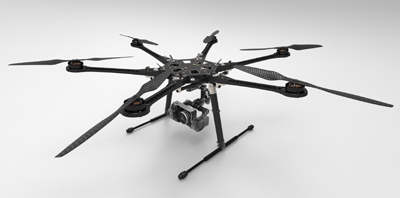
\includegraphics[scale=0.50]{DJI_S800.png}
					\caption{DJI Spreading Wings S800 \href{http://www.dji-innovations.com/wp-content/uploads/2012/05/S800_1.jpg}{[πηγή]}}
					\label{φωτ:DJI Spreading Wings S800}
			\end{figure}
			
			
			\paragraph{FreeFly Cinestar 6}{Εξάπτερο της Freefly Systems με χαρακτηριστικά την εύκολη συναρμολόγηση και την προσοχή που έχει δοθεί στη σταθερότητα του, δηλαδή στη μείωση της δόνησης που δέχεται το σύστημα της φωτογραφικής μηχανής.
			}
			\paragraph{}{Παρατίθενται δείγματα δουλειάς του συγκεκριμένου εξαπτέρου :
				\begin{itemize}
					\item \href{http://www.youtube.com/watch?v=Yo6Wdmt1zSU}{DJI video 1}
					\item \href{http://www.youtube.com/watch?v=t4ZkjpicWuo}{Payload test}
					\item \href{http://www.youtube.com/watch?v=fs1EynZ3E8o}{Cinestar 6 and Cinestar gimbal}
					\item \href{http://www.youtube.com/watch?v=J9hA6OfK9mE}{Cinestar 6}
					\item \href{http://www.youtube.com/watch?v=Bq6r-Ex6z98}{Cinestar 6 above Nab2012}
					\item \href{https://vimeo.com/47171190}{FreeFly Radian Stabiliser/Cinestar 6/Photohigher Av130/Panasonic GH2}
				\end{itemize}
			}
			\begin{figure}[hp]
					\centering
					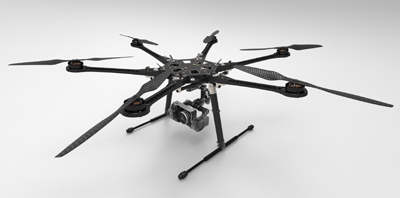
\includegraphics[scale=0.50]{DJI_S800.png}
					\caption{Cinestar 6 \href{http://www.freeflysystems.com/images/products/cinestar-6-detail.png}{[πηγή]}}
					\label{φωτ:Cinestar 6}
			\end{figure}

			\paragraph{Droidworx AD-6HL}{Εξάπτερο της Droidworx φτιαγμένο από ανθρακονήματα και σχεδιασμένο για ανύψωση αυξημένου φορτίου. Συνδυάζεται με αρκετά συστήματα αυτόματων πιλότων και παρέχει τη δυνατότητα για 360 μοίρες θέαση με το να υποστηρίζει πλατφόρμες φωτογραφικής μηχανής που ενσωματώνουν το σύστημα προσγείωσης. Όσον αφορά τις υποστηριζόμενες μηχανές αυτές είναι οι Samsung HMX-Q10, Panasonic GH2 και Canon 550d. 
			}
			\paragraph{Droidworx Skyjib 6}{Εξάπτερο της Droidworx όπως και το προηγούμενο, αλλά αποτελεί το μεγαλύτερο πολύπτερο της εταιρίας. Είναι κατασκευασμένο για να σηκώνει μέχρι και 10 κιλά (π.χ. τη μηχανή Red Epic) διατηρώντας τα υπόλοιπα πλεονεκτήματα του προηγούμενου μοντέλου.
			}
			\paragraph{}{Ένα βασικό πλεονέκτημα των δυο παραπάνω μοντέλων αποτελεί το προστατευτικό κάλυμμα το οποίο μπορεί να τοποθετηθεί στο πάνω μέρος της πλατφόρμας πτήσης.
			}
			\paragraph{}{Παρατίθενται δείγματα δουλειάς των συγκεκριμένων εξαπτέρων :
				\begin{itemize}
					\item \href{http://vimeo.com/moogaloop.swf?clip_id=29893580&server=vimeo.com&show_title=1&show_byline=1&autoplay=1}{Droidworx AD-6HLE - Hexaprod Promo Video}
					\item \href{https://vimeo.com/20411633}{Panasonic GH2 on Droidworx AD-6 Hexakopter}
					\item \href{https://vimeo.com/20921788}{FPV flight with AD6 and Panny GH2 over Steamboat Lake}
					\item \href{https://vimeo.com/42030489}{SkyJib 6X flying Red}
					\item \href{https://vimeo.com/25265975}{Droidworx CS series - flight testing}
				\end{itemize}
			}
			\begin{figure}[hp]
					\centering
					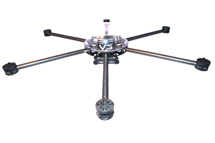
\includegraphics[scale=0.50]{Droidworx_AD_6HL.png}
					\caption{Droidworx AD-6HL \href{http://www.droidworx.com.au/shop/components/com_virtuemart/shop_image/product/AD_6_Heavy_Lift__4e2f78f506a46.jpg}{[πηγή]}}
					\label{φωτ:Droidworx AD-6HL}
			\end{figure}
			\begin{figure}[hp]
					\centering
					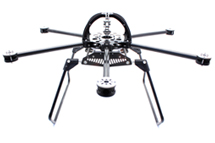
\includegraphics[scale=0.50]{Droidworx_skyjib6.png}
					\caption{Droidworx SkyJib 6 \href{http://www.droidworx.com.au/shop/components/com_virtuemart/shop_image/product/SkyJib_6_for_Ret_4f1e21acba3d6.jpg}{[πηγή]}}
					\label{φωτ:SkyJib 6}
			\end{figure}
			
			\begin{landscape}	
			\setlength\LTleft{0pt}            % default: \parindent
			\setlength\LTright{0pt}           % default: \fill
	
			\begin{longtable} { m{3cm} m{3.5cm} m{3.5cm} m{3.5cm} m{3.5cm} }
					\caption [Μοντέλα εξαπτέρων]{Μοντέλα εξαπτέρων}
					\label{πιν.:Μοντέλα εξαπτέρων}\\
					\hline
					\endfirsthead
					\multicolumn{5}{c}{συνέχεια του πίνακα \ref{πιν.:Μοντέλα εξαπτέρων}}\\
					\hline
					~\\
					\endhead
					\hline
					\multicolumn{5}{c}{ο πίνακας συνεχίζεται στην επόμενη σελίδα}\\
					\endfoot
					\multicolumn{5}{c}{ολοκληρώθηκε ο πίνακας \ref{πιν.:Μοντέλα εξαπτέρων}}\\
					\endlastfoot
					~\\
					Μοντέλο & DJI Spreading Wings S800 & Cinestar 6 & AD-6HL & SkyJib 6\\
					\hdashline
					~\\
					Κατασκευαστής & DJI Innovations & FreeFly Systems & Droidworx & Droidworx\\
					Ιστοσελίδα & \href{http://www.dji-innovations.com/products/spreading-wings-s800/overview/}{dji-innovations} & \href{http://www.freeflysystems.com/products/cinestar-6.php}{FreeFly Systems} & \href{http://www.droidworx.com.au/ADseries.html}{Droidworx} & \href{http://www.droidworx.com.au/skyjib.html}{Droidworx}\\
					\hdashline
					~\\
					\multicolumn{5}{c}{Χαρακτηριστικά}\\
					\hdashline
					βάρος απογείωσης (κιλά) & 5-7 & 5,8 (μέγιστο) & 4,2 & 6,6\\
					~\\
					βάρος φορτίου -πλατφόρμας και gimbal (κιλά) & 0-2,5 & 2,6 & 1,75 & 3\\
					~\\
					μπαταρίες & LiPo (6S, 10000mAh~15000mAh, 15C(Min)) & & & \\
					~\\
					μέγιστη κατανάλωση (watt) & 2100W & & & \\
					~\\
					κατανάλωση αιώρησης (watt) & 720W (με 6 κιλά βάρος) & & & \\
					~\\
					μέγιστος χρόνος αιώρησης (λεπτά) & 16 λεπτά (@10000mAh \& 6κιλά βάρος) & & & \\
					~\\
					προτεινόμενοι κινητήρες & περιλαμβάνονται & & AXi 2814/22 & AXi 2826/12 - (4120/20) ή ισοδύναμοι\\
					τάση τροφοδοσίας κινητήρων & 6S LiPo & & & \\
					προτεινόμενα gimbal & Zenmuse Z15 & Cinestar 3-axis & AV-200/360 - AV130/360 & AV200\\
					υποστηριζόμενες μηχανές  & Nex5-7, Panasonic GH2 & a GoPro to a Red Epic & Samsung HMX-Q10, Panasonic GH2, Canon 550d & Up to Red Scarlet class camera\\
					\hline
				\end{longtable}
				\end{landscape}
			
		\subsubsection{Οχτάπτερα}

			\paragraph{}{Στον πίνακα \ref{πιν.:Μοντέλα οχταπτέρων} παρουσιάζονται τα προτεινόμενα μοντέλα.
			}
			\paragraph{FreeFly Cinestar 8}{Αποτελεί το μεγαλύτερο μοντέλο της FreeFly ενσωματώνοντας τις τα χαρακτηριστικά και τις καινοτομίες τις εταιρίας αυτής. Παρατίθενται δείγματα δουλειάς του συγκεκριμένου οχταπτέρου :
				\begin{itemize}
					\item \href{https://vimeo.com/28738207}{CineStar 8 flies the RED EPIC}
					\item \href{https://vimeo.com/29000807}{Sony FS100 on Cinestar 8}
				\end{itemize}
			}
			\begin{figure}[hp]
					\centering
					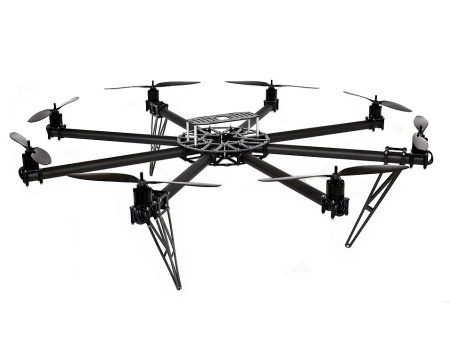
\includegraphics[scale=0.50]{cinestar_8.png}
					\caption{Cinestar 8 \href{http://www.quadrocopter.us/ready-to-fly/}{[πηγή]}}
					\label{φωτ:Cinestar 8}
			\end{figure}
			
			\paragraph{DroidWorx AD8 V3}{Η εταιρία αυτή προσφέρει οχτάπτερα μοντέλα για διάφορες εφαρμογές. Κατηγοροποιούνται ανάλογα με το βάρος που δύναται να σηκώσουν -Heavy Lift (HL), Standard Lift (SL)- και με τη δυνατότητα να περιστρέφονται γύρω από τον εαυτό τους κατά 360 μοίρες -αν έχουν τη δυνατότητα αυτή τότε το σύστημα προσγείωσης ενσωματώνεται στο gimbal. Επιλέγεται το μοντέλο AD-8HL-360.
			}
			\paragraph{}{Παρατίθενται δείγματα δουλειάς του συγκεκριμένου οχταπτέρου :
				\begin{itemize}
					\item \href{https://vimeo.com/27054891}{Octocopter in Africa}
					\item \href{https://vimeo.com/28211842}{Droidworx AD-8HLE}
					\item \href{http://www.youtube.com/watch?v=VATvkc4gc0Q}{Droidworx - AD8 HL, AV200, GoPro Hero 720p, and minus 7 Celsius}
					\item \href{http://www.youtube.com/watch?v=Q0IXjN4ckLY}{AD-8 heavy lift test}
				\end{itemize}
			}
			\begin{figure}[hp]
					\centering
					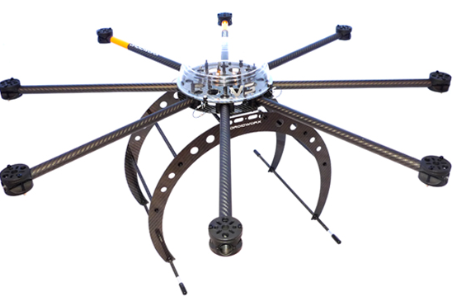
\includegraphics[scale=0.50]{DroidWorx_AD8.png}
					\caption{AD8 V3 \href{http://www.proairshop.com/media/1623/DW-AD8-HL-EXT.PNG}{[πηγή]}}
					\label{φωτ:AD8 V3}
			\end{figure}
			
			\paragraph{DroidWorx SkyJib 8}{Αποτελεί το μεγαλύτερο μοντέλο του στόλου που διαθέτει η συγκεκριμένη εταιρία. Παρατίθενται δείγματα δουλειάς του συγκεκριμένου οχταπτέρου :
				\begin{itemize}
					\item \href{http://www.youtube.com/watch?v=1v4nffpEJKk}{SkyJib 8 \& Canon EOS T2i Test}
					\item \href{http://www.youtube.com/watch?v=eKXqiZfgXcQ}{Cliffs | Skyjib 8 Aerial Video}
					\item \href{https://vimeo.com/29674297}{Droidworx SkyJib 8 with Wookong FC}
					\item \href{https://vimeo.com/28055188}{SKYJIB 8}
				\end{itemize}
			}
			\begin{figure}[hp]
					\centering
					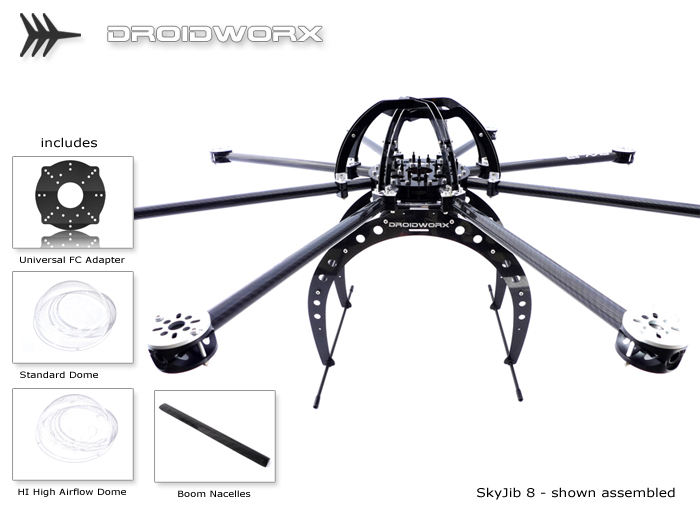
\includegraphics[scale=0.50]{DroidWrox_Skyjib8.png}
					\caption{SkyJib 8 \href{http://mikrokopter.altigator.com/images/droidworx/SkyJib-8b.jpg}{[πηγή]}}
					\label{φωτ:SkyJib 8}
			\end{figure}

			\begin{landscape}	
			\setlength\LTleft{0pt}            % default: \parindent
			\setlength\LTright{0pt}           % default: \fill
	
			\begin{longtable} { m{3cm} m{3.5cm} m{3.5cm} m{3.5cm} }
					\caption [Μοντέλα οχταπτέρων]{Μοντέλα οχταπτέρων}
					\label{πιν.:Μοντέλα οχταπτέρων}\\
					\hline
					\endfirsthead
					\multicolumn{4}{c}{συνέχεια του πίνακα \ref{πιν.:Μοντέλα οχταπτέρων}}\\
					\hline
					~\\
					\endhead
					\hline
					\multicolumn{4}{c}{ο πίνακας συνεχίζεται στην επόμενη σελίδα}\\
					\endfoot
					\multicolumn{4}{c}{ολοκληρώθηκε ο πίνακας \ref{πιν.:Μοντέλα οχταπτέρων}}\\
					\endlastfoot
					~\\
					Μοντέλο & Cinestar 8 & AD8 V3 & SkyJib 8\\
					\hdashline
					~\\
					Κατασκευαστής & FreeFly & DroidWorx & DroidWorx\\
					Ιστοσελίδα & \href{http://www.freeflysystems.com/products/cinestar-8.php}{FreeFly}  & \href{http://www.droidworx.com.au/ADseries.html}{DroidWorx} & \href{http://www.droidworx.com.au/skyjib.html}{DroidWorx}\\
					\hdashline
					~\\
					\multicolumn{4}{c}{Χαρακτηριστικά}\\
					\hdashline
					βάρος απογείωσης (κιλά) & 6,2 & 5,7 & 8,8\\
					~\\
					βάρος φορτίου -πλατφόρμας και gimbal (κιλά) & 3,05  & 2,1 & 4-5\\
					~\\
					μπαταρίες & & &\\
					~\\
					μέγιστη κατανάλωση (watt) & & &\\
					~\\
					κατανάλωση αιώρησης (watt) & & &\\
					~\\
					μέγιστος χρόνος αιώρησης (λεπτά) & & &\\
					~\\
					προτεινόμενοι κινητήρες & & AXi- 2814/22 & AX i2826/12 - (4120/20) ή ισοδύναμοι\\
					τάση τροφοδοσίας κινητήρων &  & &\\
					προτεινόμενα gimbal & Cinestar 3-axis & AV-200/360, AV130/360 & AV200\\
					υποστηριζόμενες μηχανές  & a GoPro to a Red Epic (GH2, FS100, T2i) & Samsung HMX-Q10, Panasonic GH2, Canon 5/7D & Up tp Red Epic class video camera\\
					\hline
				\end{longtable}
				\end{landscape}	
			
		\subsection{Αυτόματος πιλότος και χειριστήριο εδάφους}
		
			\subsubsection{Αυτόματος πιλότος}
			\paragraph{}{Για την εξασφάλιση τόσο της ασφάλειας πολυπτέρου και περιβάλλοντος, όσο και της ποιότητας του αποτελέσματος κρίνεται απαραίτητος. Διαθέτοντας αυτόν, το πολύπτερο μπορεί να αιωρείται μόνο του χωρίς την παρέμβαση του ανθρώπου από το έδαφος, ελαχιστοποιώντας με αυτόν τον τρόπο τις αναταράξεις που μπορεί να επιφέρει η χειροκίνητη καθοδήγηση. Επίσης, σημαντικό αποτελεί το γεγονός ότι χάνοντας το σήμα δεν καταρρίπτεται αλλά διατηρεί το ύψος ή/και την πορεία του. Επιπλέον, δύναται να προγραμματιστεί ώστε να επιστρέφει αυτόματα ύστερα από κάποια δεύτερα. Τέλος, στο ίδιο μοτίβο, σε περίπτωση που οι μπαταρίες αδειάσουν, επιστρέφει σε προκαθορισμένο σημείο προσγείωσης με ασφάλεια.
			}
			\paragraph{}{Υπάρχουν εταιρίες που προσφέρουν ολοκληρωμένα συστήματα αυτόματου πιλότου τα οποία διαφοροποιούνται στην ποιότητα τους -στο πόσο σταθερό είναι το πολύπτερο στον αέρα- και στις λειτουργίες που ενσωματώνουν δίνοντας ιδιαίτερη έμφαση στην αυτόματες διαδικασίες ασφάλειας.
			}
			\paragraph{}{Στον πίνακα \ref{πιν.:Μοντέλα αυτόματων πιλότων} παρουσιάζονται τα προτεινόμενα μοντέλα.
			}
			
			\paragraph{Zero YS-X6}{Παρατίθενται δείγματα δουλειάς του συγκεκριμένου πιλότου :
				\begin{itemize}
					\item \href{http://www.youtube.com/watch?v=r1_O_VvFZ1U}{Zero YS-X6 10km/h test}
					\item \href{http://www.youtube.com/watch?v=JRiiGby-e-4}{Zero YS-X6}					
				\end{itemize}
			}
			
			\paragraph{DJI Wookong-M}{Αποτελεί ένα πλήρες σύστημα αυτοματοποιημένης πτήσης. Διαθέτει τρία mode πτήσης. Το Gps-Atti όντας απόλυτα αυτόματο από την απογείωση μέχρι και την προσγείωση ή το Atti το οποίο αφορά χειροκίνητο χειρισμό με ενεργοποιημένο το σταθεροποιητή πτήσης και τέλος την πλήρως χειροκίνητη πτήση χωρίς καμία βοήθεια.
			}
			\paragraph{}{Παρατίθενται δείγματα δουλειάς του συγκεκριμένου πιλότου :
				\begin{itemize}
					\item \href{https://vimeo.com/38972821}{DJI Wookong-M}
					\item \href{https://vimeo.com/43035644}{Droidworx ADX3 HL, DJI Wookong}
					\item \href{https://vimeo.com/40803086}{DJI Wookong 4S Test 1}			
				\end{itemize}
			}
			
			\paragraph{Feiyu Tech FY-91Q}{Ο συγκεκριμένος πιλότος έχει ως μεγάλο πλεονέκτημα την τιμή του, αλλά δυστυχώς δεν διαθέτει αρκετές λειτουργίες καθώς και μονάδα τροφοδοσίας. Παρατίθενται δείγματα δουλειάς του συγκεκριμένου πιλότου :
				\begin{itemize}
					\item \href{https://vimeo.com/27469866}{FY91Q Kiso river}
					\item \href{http://www.youtube.com/watch?v=5JWZVufFHKQ}{FY-91Q GoPro}
				\end{itemize}
			}
			
			\paragraph{HoverflyPRO}{Παρατίθενται δείγματα δουλειάς του συγκεκριμένου πιλότου :
				\begin{itemize}
					\item \href{https://vimeo.com/26895602#}{Guam helicopter aerials}
					\item \href{http://www.youtube.com/watch?v=b0fwnqsdI8w}{Aerial Video - Aspen Trees}
					\item \href{https://vimeo.com/29466533#}{Got Aerial and Aerial Exposure}
				\end{itemize}
			}
			
			\begin{landscape}	
			\setlength\LTleft{0pt}            % default: \parindent
			\setlength\LTright{0pt}           % default: \fill
	
			\begin{longtable} { m{3cm} m{3.5cm} m{3.5cm} m{3.5cm} m{3.5cm} }
					\caption [Μοντέλα αυτόματων πιλότων]{Μοντέλα αυτόματων πιλότων}
					\label{πιν.:Μοντέλα αυτόματων πιλότων}\\
					\hline
					\endfirsthead
					\multicolumn{5}{c}{συνέχεια του πίνακα \ref{πιν.:Μοντέλα αυτόματων πιλότων}}\\
					\hline
					~\\
					\endhead
					\hline
					\multicolumn{5}{c}{ο πίνακας συνεχίζεται στην επόμενη σελίδα}\\
					\endfoot
					\multicolumn{5}{c}{ολοκληρώθηκε ο πίνακας \ref{πιν.:Μοντέλα αυτόματων πιλότων}}\\
					\endlastfoot
					~\\
					Μοντέλο & Zero YS-X6 GU-INS & DJI Wookong-M & Feiyu Tech FY-91Q & HoverflyPRO\\
					\hline
					~\\
					Κατασκευαστής & Zero & DJI Innovations & Feiyu Tech & Hoverfly\\
					Ιστοσελίδα & \href{http://www.zerouav.net/productmore.aspx?id=82}{Zero} & \href{http://www.dji-innovations.com/products/wookong-m/overview/}{dji-innovations} & \href{http://www.feiyu-tech.com/product-en.php?id=12&mlist=3&}{Feiyu Tech} & \href{http://www.feiyu-tech.com/product-en.php?id=12&mlist=3&}{Hoverfly}\\
					\hline
					~\\
					\multicolumn{5}{c}{Χαρακτηριστικά}\\
					\hdashline
					Υποστηριζόμενα πολύπτερα & 4, 6, 8 & 4, 6, 8 & 4, 6 & 4, 6, 8\\
					\hdashline
					~\\
					Τύπος υποστηριζόμενου δέκτη & Normal, Futaba, Sbus & JR, Futaba, Hitec, S-Bus, PPM & & Typical RC Receiver\\
					\hdashline
					~\\
					Τύπος υποστηριζόμενου πομπού & PCM, 2.4GHz, S-Bus & PCM or 2.4GHz with minimum 7 channels and Failsafe function available on all channels & Robbe-Futaba (PPM, PCM 1024, PCM G3 mode, 2.4 GHz systems), Graupner-JR (PPM 8, PPM 12, SPCM mode), MPX (PPM8, PPM 12 with UNI mode) & HiTec, Spektrum, JR, Futaba (it needs 5 channels)\\
					\hdashline
					~\\
					\multicolumn{5}{c}{Διαστάσεις}\\
					\hdashline
					~\\
					Πρωτεύων ελεγκτής (μμ) & 60x90 & 51,2x38x15,3 & 55x33x20 & 70x70x12.7\\
					~\\
					IMU (μμ) & 40x45 & 41,4x31,1x27,8 & ενσωματώνεται στον ελεγκτή & ενσωματώνεται στον ελεγκτή\\
					~\\
					GPS-Compass (μμ) & 55x12 & 50x9 & 55x33x20 & 70x70x12.7\\
					~\\
					Wifi 2.4ghz (μμ) & 42x67 & & δεν διαθέτει & δεν διαθέτει\\
					~\\
					Led (μμ) & & 25x25x7 & δεν διαθέτει & δεν διαθέτει\\
					~\\
					Power unit (μμ) & & 39,5x27,5x9,7 & δεν διαθέτει & δεν διαθέτει\\
					\hdashline
					~\\
					Βάρος (γραμμάρια) & 180 & <= 118 & 40 & 70\\
					\hdashline
					~\\
					Συχνότητα & 400MHz & 400MHz & 400MHz & \\
					\hdashline
					~\\
					Θερμοκρασία λειτουργίας (celsius) & & -5 to 60 & -25 to 70 & \\
					\hdashline
					~\\
					Mode λειτουργίας & Manual, Attitude, GPS attitude & Manual, Attitude, GPS attitude & Stabilized Mode, Automated Hover Hold, Automated Return to Home Mode & Auto-Leveling, Altitude Hold\\
					\hdashline
					~\\
					Μέγιστη γωνιακή ταχύτητα (deg/s) & 300  & & & \\
					\hdashline
					~\\
					\multicolumn{5}{c}{Ακρίβεια αιώρησης}\\
					~\\
					κάθετα (μ) & 0,5 & 0,5 & & \\
					~\\
					οριζόντια (μ) & 2 & 2 & 1,5 & \\
					\hdashline
					~\\
					Μέγιστη yaw γωνιακή ταχύτητα (deg/s) & 180 & 150  & & \\
					\hdashline
					~\\
					Μέγιστη γωνία tilt (μοίρες) & 25 & 35 & & \\
					\hdashline
					~\\
					Μέγιστη οριζόντια ταχύτητα &  & & & \\
					\hdashline
					~\\
					Μέγιστη κάθετη ταχύτητα (m/s) & 4 & 6 & & \\
					\hdashline
					~\\
					Λειτουργίες ασφαλείας & Auto Hover mode, Auto Navigation mode, Auto Go Home, Low voltage alarm via phone/tablet & 2 level Low Voltage Protection, Hover, Go-home, Altitude Go-home, Attitute controllable when one power output failed & & Return-to-Home\\
					\hdashline
					~\\
					Επιτρεπτές συνθήκες ανέμου & - 8m/s(28.2km/h) & < 8m/s (17.9mph/28.8km/h) & & \\
					\hdashline
					~\\
					Επιπλέον λειτουργίες & Follow me (with a phone having gps), Auto take off-landing, Waypoint navigation (limit 4 points, within 200m diameter), Point of interest & Auto take off-landing, Point of interest & & Data Logging\\
					\hdashline
					~\\
					Μπαταρίες & 3-6s lipo & 2S~6S LiPo & 5Volt είσοδος & 2S~5S LiPo\\
					\hdashline
					~\\
					Κατανάλωση & & MAX 5W (0.9A@5V, 0.7A@5.8V,0.5A@7.4V,0.4A@8V) & & \\
					\hline
				\end{longtable}
				\end{landscape}

		
		\subsubsection{Xειροκίνητη πτήση}
			\paragraph{}{Συνήθως αποτελείται από ένα χειριστήριο και ένα δέκτη τοποθετούμενο στην πλατφόρμα πτήσης. Ο χειριστής θα μπορεί να καθορίζει σε πραγματικό χρόνο την πορεία του πολυπτέρου και να το κατευθύνει κατά την επιθυμία του.
			}
			\paragraph{}{Υπάρχουν ποικίλα μοντέλα που ικανοποιούν τις απαιτήσεις μας. Συγκεκριμένα χρειαζόμαστε ένα από τα JR, Futaba, Hitec, S-Bus ή PPM στα 2,4 GHz με 7 κανάλια τουλάχιστον και κάθε κανάλι να προσφέρει λειτουργίες ασφαλείας. Αυτά λειτουργούν σε ένα ευρύ φάσμα συχνοτήτων -72 MHz, FM, PCM, G3 και 2,4 GHz.
			}
			
		\subsection{Επίγειος σταθμός παρατήρησης και ελέγχου πτήσης}
			\paragraph{}{Αποτελεί συσκευή που ενσωματώνει επιπλέον δυνατότητες παρακολούθησης της πτήσης και επέμβασης σε αυτήν. Μπορεί να διαθέτει ειδικό λογισμικό με το οποίο να αποτυπώνεται η πορεία του σε χάρτη (π.χ. google maps) και με το οποίο μπορούν να δοθούν κρίσιμες εντολές όπως άμεση προσεδάφιση, επιστροφή στο σπίτι κ.λ.π.. Επιπλέον μπορεί να διαθέτει λειτουργία OSD -on screen data, δεδομένα στην οθόνη. Δηλαδή, λαμβάνεται βίντεο της πτήσης από την οπτική του πολυπτέρου και επιπλέον απεικονίζονται και διάφορα σημαντικά δεδομένα, όπως υψόμετρο, ταχύτητα ανέμου, ταχύτητα πολυπτέρου κ.λ.π..
			}
			\paragraph{Το σύστημα αυτό δεν θα αναλυθεί στην έκδοση αυτή του κειμένου.}{Απλώς αναφέρεται ότι από τους προαναφερθέντες αυτόματους πιλότους ο DJI Wookong-M διαθέτει έξτρα κεραία και λογισμικό για την καθοδήγηση και την OSD παρατήρηση του πολυπτέρου από το σταθμό αυτό. Ο Zero YS-X6 GU-INS διαθέτει μέσα στο αρχικό πακέτο την κεραία και το αντίστοιχο λογισμικό. Ο Feiyu Tech FY-91Q απαιτεί ξεχωριστό εξάρτημα για την OSD παρέχοντας και το λογισμικό παρατήρησης και καθοδήγησης. Τέλος, ο HoverFly ενσωματώνει τη λειτουργία OSD αλλά δεν παρέχει αντίστοιχο λογισμικό. Επιτρέπει απλώς την παρατήρηση της πτήσης μέσω της παράθεσης των δεδομένων (ύψος, ταχύτητα, κ.λ.π.) με το βίντεο που καταγράφει η κάμερα.
			}
			
			
		\section{Σύστημα λήψης εικόνας}
		
		\subsubsection{Πλατφόρμα της μηχανής}
			\paragraph{}{Στα αγγλικά χρησιμοποιείται ο όρος "gimbal". Αποτελεί το σημείο στήριξης της μηχανής πάνω στην πλατφόρμα πτήσης. Είναι υπεύθυνο για το είδος και μέγεθος της μηχανής, τις επιτρεπτές κινήσεις που μπορεί να εκτελέσει η μηχανή καθώς και για τις δυνατές γωνίες λήψεις. Οι δυνατές κινήσεις είναι η περιστροφή στον κάθετο άξονα -tilt, κίνηση πάνω κάτω- η περιστροφή στον οριζόντιο άξονα -pan, κίνηση δεξιά αριστερά- και η περιστροφή γύρω από τον εαυτό της -roll. Όσο μεγαλύτερο το εύρος των κινήσεων αυτών, τόσο το καλύτερο.
			}
			
			\begin{landscape}	
			\setlength\LTleft{0pt}            % default: \parindent
			\setlength\LTright{0pt}           % default: \fill
	
			\begin{longtable} { m{3cm} m{3.5cm} m{3.5cm} m{3.5cm}}
					\caption [Μοντέλα gimbal]{Μοντέλα gimbal}
					\label{πιν.:Μοντέλα gimbal}\\
					\hline
					\endfirsthead
					\multicolumn{4}{c}{συνέχεια του πίνακα \ref{πιν.:Μοντέλα gimbal}}\\
					\hline
					~\\
					\endhead
					\hline
					\multicolumn{4}{c}{ο πίνακας συνεχίζεται στην επόμενη σελίδα}\\
					\endfoot
					\multicolumn{4}{c}{ολοκληρώθηκε ο πίνακας \ref{πιν.:Μοντέλα gimbal}}\\
					\endlastfoot
					~\\
					Μοντέλο & DJI Zenmuse Z15 & Cinestar 3 Axis & AV200 + 360 pan V3\\
					\hline
					~\\
					Κατασκευαστής & DJI Innovations & Freefly Systems & PhotoHigher\\
					Ιστοσελίδα & \href{http://www.dji-innovations.com/products/zenmuse-z15/overview/}{dji-innovations} & \href{http://www.freeflysystems.com/products/cinestar-3-axis-gimbal.php}{Cinestar} & \href{http://photohigher.co.nz/products/camera-gimbals-and-kits/av200-pan-360-with-skids/}{PhotoHigher}\\
					\hline
					~\\
					\multicolumn{4}{c}{Χαρακτηριστικά}\\
					\hdashline
					Τύπος υποστηριζόμενου δέκτη & S-Bus  & δεν διαθέτει σταθεροποιητή & δεν διαθέτει σταθεροποιητή\\
					\hdashline
					Τύπος υποστηριζόμενου πομπού & Four spare receiver channels & δεν διαθέτει σταθεροποιητή & δεν διαθέτει σταθεροποιητή\\
					\hdashline
					Mode λειτουργίας & Orientation-locked control, Non orientation-locked control, FPV mode (Reset) & δεν διαθέτει σταθεροποιητή & δεν διαθέτει σταθεροποιητή\\
					\hdashline
					Μέγιστη ταχύτητα περιστροφής & & & \\
					Pan axis (deg/s) & $\pm$130 & & \\
					Tilt axis  (deg/s) & $\pm$130 & & \\
					Roll axis (deg/s) & $\pm$30 & & \\
					\hdashline
					Εύρος περιστροφής & & & \\
					Pan axis control (μοίρες) & $\pm$360 continuous rotation & & 360\\
					Tilt axis control (μοίρες) & $\pm$360 continuous rotation & & 180\\
					Roll axis control (μοίρες) & $\pm$40 ($\pm$360 mechanic continuous rotation) & & $\pm$35\\
					\hdashline
					Ασύρματος χειρισμός μηχανής & Camera shutter control support & δεν διαθέτει σταθεροποιητή & δεν διαθέτει σταθεροποιητή\\
					\hdashline
					Υποστηριζόμενες μηχανές & SONY Nex-5N/Nex-7, Panasonic GH-2 & a GoPro to a Red Epic & Canon 5Dmk2 or 7D\\
					\hdashline
					Υποστηριζόμενοι αυτόματοι πιλότοι & διαθέτει ενσωματωμένο & δεν διαθέτει & δεν διαθέτει\\
					\hdashline
					Επιπλέον λειτουργίες & HDMI-AV module, Wireless video transmission support & δεν διαθέτει & δεν διαθέτει\\
					\hdashline
					Σύστημα προσγείωσης & δεν διαθέτει & προαιρετικό & προαιρετικό\\
					\hdashline
					Θερμοκρασία λειτουργίας (Celsius) & -10-50 & & \\
					\hline
				\end{longtable}
				\end{landscape}
			
		\subsubsection{Αυτόματος πιλότος για την πλατφόρμα της μηχανής}
			\paragraph{}{Αποτελεί απαραίτητο υποσύστημα εφόσον αναλαμβάνει το ρόλο του σταθεροποιητή του gimbal ενάντια στις διάφορες αναταράξεις που δέχεται η κάμερα. Φροντίζει, λοιπόν, να παραμένει η κάμερα στο επιθυμητό σημείο ανεξάρτητα από την κίνηση του πολυπτέρου. Εν παραδείγματι, έστω ότι χρησιμοποιούμε τη λειτουργία που μας επιτρέπει η κάμερα να κρατάει σταθερή θέση σε σχέση με το πολύπτερο. Ο σταθεροποιητής φροντίζει για αυτό -να μην αλλάζει η σχετική θέση πολυπτέρου - κάμερας. Επιπλέον, φροντίζει κάθε μετάβαση της κάμερας, αυτόματη ή μη, να γίνεται με τον πλέον ομαλό τρόπο. Χρησιμοποιώντας τον αυτόματο πιλότο του gimbal λαμβάνουμε εξαιρετικής ποιότητας λήψεις χωρίς κουνήματα ή "δόντι" στην εικόνα.
			}
			\paragraph{}{Στην αγορά δεν υπάρχουν πολλά έτοιμα συστήματα προς επιλογή. Είναι λιγότερα από δέκα (10) και από αυτά λίγα καλύπτουν τις απαιτήσεις που έχουν τεθεί. Ξεχωρίζουν τα συστήματα της DJI -είναι ενσωματωμένο στο αντίστοιχο gimbal και συνεργάζεται μόνο με αυτό- της Freefly -ονομάζεται Radian και χρειάζεται μία μονάδα ανά άξονα- της Hoverfly - ονομάζεται Hoverfly Gimbal και αποτελεί έναν αξιόλογο σταθεροποιητή.
			}
			
			\begin{landscape}	
			\setlength\LTleft{0pt}            % default: \parindent
			\setlength\LTright{0pt}           % default: \fill
	
			\begin{longtable} { m{3cm} m{3cm} m{3cm} m{3cm} m{3cm} m{3cm} }
					\caption [Μοντέλα αυτόματου πιλότου gimbal]{Μοντέλα αυτόματου πιλότου gimbal}
					\label{πιν.:Μοντέλα αυτόματου πιλότου gimbal}\\
					\hline
					\endfirsthead
					\multicolumn{6}{c}{συνέχεια του πίνακα \ref{πιν.:Μοντέλα αυτόματου πιλότου gimbal}}\\
					\hline
					~\\
					\endhead
					\hline
					\multicolumn{6}{c}{ο πίνακας συνεχίζεται στην επόμενη σελίδα}\\
					\endfoot
					\multicolumn{6}{c}{ολοκληρώθηκε ο πίνακας \ref{πιν.:Μοντέλα αυτόματου πιλότου gimbal}}\\
					\endlastfoot
					~\\
					Μοντέλο & DJI Zenmuse Z15 & Freefly Radian & Skyline Gyro RSGS & Hoverfly Gimbal & PicLoc 3X Pro\\
					\hline
					~\\
					Κατασκευαστής & DJI & Freefly Systems & Photohigher & HoverFly & RotorPics\\
					Ιστοσελίδα & \href{http://www.dji-innovations.com/products/zenmuse-z15/overview/}{dji-innovations} & \href{http://www.freeflysystems.com/products/freefly-radian.php}{dji-innovations} & \href{http://photohigher.co.nz/products/flight-and-gimbal-control-systems/skyline-gyro-rsgs/}{Photohigher} & \href{http://www.hoverflytech.com/gimbal_1WNK.html}{HoverFly} & \href{http://www.rotorpics.com/}{RotorPics}\\
					\hline
					~\\
					\multicolumn{6}{c}{Χαρακτηριστικά}\\
					\hdashline
					Άξονες ελέγχου & Pan, Tilt, Roll & Pan, Tilt, Roll & Pan, Tilt, Roll (Υπάρχουν προβλήματα με την σταθεροποίηση του pan. Αναμένεται firmware) & Pan, Tilt, Roll & Pan, Tilt, Roll\\
					\hdashline
					Τύπος υποστηριζόμενου δέκτη & Futaga, Hitec, JR & S.bus, PPM, PWM, and spektrum & PPM, PWM, S.Bus or Spektrum & & \\
					\hdashline
					Τύπος υποστηριζόμενου πομπού & Futaga, Hitec, JR (8 channels) & προτείνεται πομπός οχτώ καναλιών & & τυπικός με τρία κανάλια (π.χ. Spektrum DX8) & Futaba or JR (or Compatible systems with 1500us center) (8/9 channel control with 3 sliders or rotary knobs)\\
					\hdashline
					Mode λειτουργίας & Orientation-locked control, Non orientation-locked control, FPV mode (Reset) & Off, Fixed position stabilized, Stabilized slew & & Autonomous mode, Guided mode & Slew or Proportional control mode\\
					\hdashline
					Ασύρματος έλεγχος & roll, tilt and pan axis control, working Mode switch, camera shutter control, HDMI switch, Gimbal orientation (down or forward) switch in FPV Mode & & & Angle position, Angle velocity, Mode switch, Auto compensation, & Slew or Proportional mount control, Remote Mount Control, Remote Gain Control\\
					\hdashline
					Ασύρματος χειρισμός μηχανής & Camera shutter control support & δεν διαθέτει & & δεν διαθέτει & δεν διαθέτει\\
					\hdashline
					Υποστηριζόμενες μηχανές & SONY Nex-5N/Nex-7, Panasonic GH-2 & a GoPro to a Red Epic & Canon 5Dmk2 or 7D & δεν συνδέεται με κάποια & δεν συνδέεται με κάποια\\
					\hdashline
					Υποστηριζόμενοι κινητήρες & ενσωματώνεται σε συγκεκριμένο gimbal & 1520us, 760us & & & τυπικοί αναλογικοί και ψηφιακοί κινητήρες\\
					Υποστηριζόμενη συχνότητα κινητήρων  & ενσωματώνεται σε συγκεκριμένο gimbal & 4 επίπεδα μέχρι 400Hz & & & 4 διαφορετικές συχνότητες, μέχρι 560Hz\\
					\hdashline
					Τρόπος ενσωμάτωσης & μία μονάδα στο σύνολο & μία μονάδα ανά άξονα & μία μονάδα ανά άξονα & μία μονάδα στο σύνολο & μία μονάδα ανά άξονα\\
					\hdashline
					Επιπλέον λειτουργίες & HDMI-AV module, Wireless video transmission support & δεν διαθέτει & δεν διαθέτει & δεν διαθέτει & AutoPanorama mode \\
					\hdashline
					Βάρος (γραμμάρια) & & & & & 40\\
					\hdashline
					Διαστάσεις (μμ) & & & & 45x45x15 & 36x28x19\\
					\hdashline
					Θερμοκρασία λειτουργίας (Celsius) & -10-50 & & & & 0-40\\
					\hline
				\end{longtable}
				\end{landscape}
			
			
		\subsubsection{Επίγειος σταθμός ελέγχου της πλατφόρμας της μηχανής}
			\paragraph{}{Αποτελείται από ένα πομπό τοποθετούμενο στο έδαφος και ένα δέκτη τοποθετούμενο στο πολύπτερο. Ο πομπός συνήθως είναι ένα χειριστήριο που ενσωματώνει τις απαραίτητες λειτουργίες, δηλαδή την περιστροφή της πλατφόρμας της μηχανής, συνεπώς την αλλαγή των γωνιών θέασης.
			}
			\paragraph{}{Υπάρχουν ποικίλα μοντέλα που ικανοποιούν τις απαιτήσεις μας. Συγκεκριμένα χρειαζόμαστε ένα από τα JR, Futaba, Hitec, S-Bus ή PPM στα 2,4Ghz με 4 έως 9 κανάλια ανάλογα με τον επιλεχθέντα σταθεροποιητή.
			}
		
		\subsubsection{Μηχανή}
			\paragraph{}{Η μηχανή λήψης εικόνας. Για μεγαλύτερη ποιότητα είναι απαραίτητο να τραβάει υψηλής ανάλυσης εικόνα και βίντεο (hd) καθώς και να διαθέτει μεγάλη χωρητικότητα για μεγαλύτερης διάρκεια γύρισμα.
			}
			\paragraph{}{Διαθέτουμε ήδη μία Canon 550D, μία Panasonic AG-HPX200 και μία GoPro. Επιπλέον, αποδεκτές λύσεις αποτελούν και οι Sony nex7 και Panasonic GH2 οι οποίες απαιτούνται από το gimbal της Dji.
			}
		
		\subsubsection{Σταθμός ελέγχου της μηχανής}	
			\paragraph{}{Επιπλέον, απαραίτητο είναι και το σύστημα με το οποίο θα ελέγχουμε τις λειτουργίες της μηχανής από το έδαφος. Συγκεκριμένα, είναι επιθυμητό να μπορούμε να εναλλάσσουμε τις λειτουργίες φωτογραφικής μηχανής και κινηματογράφησης, να ενεργοποιούμε το φλας, να επιλέγουμε την αρχή και το τέλος της κινηματογράφησης και τέλος την λειτουργία του zoom.
			}
			\paragraph{}{Οι φωτογραφικές μηχανές που έχουν αναφερθεί παραπάνω υλοποιούν βασικές λειτουργίες απομακρυσμένης διαχείρισης -ενσύρματη ή ασύρματη. Ενδεικτικά η sony nex7 ελέγχεται μέσω υπερύθρου αισθητήρα. Αντίθετα η panasonic GH-2 ελέγχεται μέσω καλωδίου. Τέλος η canon 550D υποστηρίζει και τις δύο μεθόδους. Όμως τα ασύρματα χειριστήρια των μηχανών αυτών δεν έχουν σχεδιαστεί με σκοπό την εναέρια λήψη. Συνεπώς, πρέπει να κατασκευαστεί ένα σύστημα που θα αποτελείται από έναν ασύρματο ελεγκτή τοποθετημένο μαζί με τη μηχανή και έναν επίγειο πομπό. Με σκοπό την μικρότερη επιβάρυνση του υπόλοιπου συστήματος, σκοπεύεται να ενσωματωθεί το εν λόγω σύστημα στο σύστημα ασύρματου ελέγχου της πλατφόρμας της μηχανής, δηλαδή το ο επίγειος έλεγχος να πραγματοποιείται διαμέσου του χειριστηρίου για την περιστροφή της μηχανής και ο ελεγκτής που θα βρίσκεται στο πολύπτερο να συνδεθεί με τον αντίστοιχο δέκτη. Υπάρχουν διάφορα εξαρτήματα αυτού του σκοπού, με τα πιο ενδιαφέροντα που ανακαλύψαμε να είναι τα δύο ακόλουθα.
			}
			\paragraph{StratoSnapper}{Όπως αναφέρεται στην \href{http://littlesmartthings.com/stratosnapper/}{ιστοσελίδα} του, μπορεί να ελέγξει μία μηχανή μέσω υπερύθρων ή μέσω καλωδίου στο οποίο όμως πρέπει να συνδέσουμε την υποδοχή που ταιριάζει στη μηχανή μας. Επιπλέον, διαθέτει δύο εισόδους ελέγχου κινητήρων στις οποίες συνδέεται ο ασύρματος δέκτης (π.χ. spectrum receiver). Από τις αναφερθείσες φωτογραφικές μηχανές υποστηρίζει τον έλεγχο του φλας και του βίντεο για τη canon (in live view mode) 550D και τις sony nex 5 και 7\footnote{Για την πλήρη λίστα των υποστηριζόμενων μηχανών ανατρέξατε στην \href{http://littlesmartthings.com/stratosnapper-supported-cameras/}{ιστοσελίδα}}. Για τις λειτουργίες αυτές αφιερώνει δύο κανάλια. Με το πρώτο ελέγχεται το φλας και με το δεύτερο η λειτουργία του βίντεο. Επισημαίνεται ότι το βάρος είναι μόλις 6 γραμμάρια και το μέγεθός του 26x34μμ.
			}
			\paragraph{CAMremote-2A}{Κατασκευάζεται από την VP-Systems (\href{http://vp-systems.eu/camremote.html}{ιστοσελίδα}) και μπορεί αν ελέγξει το φλας, το zoom, την ταχύτητα του κλείστρου κ.ά. Επιπλέον, διαθέτει χρονόμετρο για την λειτουργία της μηχανής με καθυστέρηση. Ελέγχει φωτογραφικές μηχανές οι οποίες υποστηρίζουν απομακρυσμένο έλεγχο μέσω usb θύρας, υπέρυθρων ακτίνων ή καλωδίου. Από την άλλη συνδέεται με όλους τους τυπικούς ασύρματους δέκτες όπως οι JR, Futaba και Hitech. Απαιτεί δύο με τρία κανάλια για τις υποστηριζόμενες λειτουργίες. Αναφορικά με τις προαναφερθείσες μηχανές (canon, sony και panasonic) μπορεί να συνεργαστεί με όλες. Τέλος, αξιοσημείωτα είναι το μέγεθός του (31x21μμ), το βάρος του (3 γραμμάρια) και η κατανάλωση ρεύματος (1-25 mA).
			}
		
		
		\subsubsection{Εναέριος σταθμός μετάδοσης εικόνας}	
			\paragraph{}{Αποτελεί τη συσκευή που μεταδίδει την εικόνα που "βλέπει" η μηχανή με σκοπό να τη λήψη της από επίγειες συσκευές. Θα πρέπει η μετάδοση να είναι ομαλή και απρόσκοπτη και εφικτή για μεγάλες αποστάσεις, χωρίς να είναι απαραίτητη η ορατή ζεύξη. Θα πρέπει να λαμβάνει υπόψιν τους περιορισμούς μετάδοσης σήματος σε ανοιχτούς χώρους.
			}
		
		\subsubsection{Επίγειος σταθμός λήψης σύγχρονης εικόνας}	
			\paragraph{}{Αποτελεί τη συσκευή με την οποία λαμβάνεται η εικόνα που βλέπει η μηχανή στον αέρα και σύμφωνα με την οποία δρα αναλόγως ο χρήστης της μηχανής. Δηλαδή τραβάει ή όχι φωτογραφίες και βίντεο και τροποποιεί κατά βούληση τη γωνία θέασης.
			}
			\paragraph{}{Το σύστημα αυτό δεν θα αναλυθεί στην παρούσα έκδοση του κειμένου.}
			
		\subsubsection{Επίγειος σταθμός καταγραφής σύγχρονης εικόνας}
			\paragraph{}{Αποτελεί τη συσκευή η οποία επιτρέπει την καταγραφή εικόνας σε υψηλή ανάλυση (hd). Η μονάδα αποθήκευσης θα πρέπει να εξυπηρετεί τις ανάγκες των γυρισμάτων για μεγάλος πλήθος φωτογραφιών και πολύωρου βίντεο.
			}
			\paragraph{}{Το σύστημα αυτό δεν θα αναλυθεί στην παρούσα έκδοση του κειμένου.}
	
	\chapter{Νομική ανάλυση}
		
		\paragraph{}{Για να ολοκληρώσουμε την κατασκευή του συστήματος εναέριας φωτογράφησης και κινηματογράφησης θα πρέπει να γνωρίζουμε τους περιορισμούς που θέτει ο νομοθέτης αφενός για τη χρήση των μη επανδρωμένων αεροναυτικών οχημάτων και αφετέρου για τα συστήματα από τα οποία αποτελείται το πολύπτερο. Συγκεκριμένα, το πεδίο το οποίο οφείλεται να διερευνηθεί είναι η τηλεπικοινωνιακή ζεύξη του πολυπτέρου με τους επίγειους σταθμούς. 
			}
			
		\section{Νομικό πλαίσιο αερομοντέλων και μη επανδρωμένων αεροναυτικών οχημάτων}
			
			\paragraph{}{Ο κυριότερος κανονισμός που διέπει την πτήση των αερομοντέλων έχει συνταχθεί από τον διοικητή της ΥΠΑ (υπηρεσία πολιτικής αεροπορίας) και έχει δημοσιευτεί στην εφημερίδα της κυβέρνησης τον Ιανουάριο του 2010 - ΦΕΚ 2010Β9 \cite{ΦΕΚ2010Β9}.
			}
			\paragraph{}{Σύμφωνα με αυτόν διακρίνουμε τους εξής τύπους ιπτάμενων μοντέλων :
			\begin{quote}
				\textbf{Αερομοντέλο ή Μοντέλο Αεροσκάφους (Model Aircraft)} είναι μία ιπτάμενη συσκευή περιορισμένων διαστάσεων, που φέρει ή όχι προωθητικό σύστημα, που δεν έχει τη δυνατότητα να μεταφέρει άνθρωπο, και το οποίο χρησιμοποιείται για αεραθλητισμό ή ψυχαγωγία. Τα αερομοντέλα μπορεί να έχουν τη μορφή αεροπλάνου, ανεμοπτέρου, ελικοπτέρου, αυτόγυρου, υδροπλάνου, αμφίβιου, αλεξίπτωτου, αερόστατου, αερόπλοιου, ή άλλης μορφής. Τα αερομοντέλα μπορεί να είναι τηλεχειριζόμενα, ελεύθερης πτήσης, ή κυκλικής πτήσης.\linebreak
				\textbf{Μη επανδρωμένο αεροναυτικό όχημα (UAV - Unmanned Aeronautical Vehicle)} είναι μία ιπτάμενη συσκευή που δεν μεταφέρει άνθρωπο, και το οποίο έχει αναπτυχθεί και χρησιμοποιείται για επιστημονικούς, ερευνητικούς ή στρατιωτικούς σκοπούς. Τα UAV δεν θεωρούνται αερομοντέλα, και τα αερομοντέλα δεν θεωρούνται UAV.			
			\end{quote}
			}
			\paragraph{}{Επιπλέον ο εν λόγω κανονισμός χωρίζει τα αερομοντέλα και τα uav σε δύο κατηγορίες λαμβάνοντας με κριτήριο το βάρος τους.
			\begin{quote}
				\textbf{Κατηγορία Α'}: Περιλαμβάνει τα αερομοντέλα με συνολική μάζα απογείωσης μικρότερη ή ίση των 7.000 γραμμαρίων (7kg).\linebreak
				\textbf{Κατηγορία Β'}: Περιλαμβάνει τα αερομοντέλα με συνολική μάζα απογείωσης μεγαλύτερη των 7.000 γραμμαρίων (7kg) και μέχρι 25.000 γραμμαρίων (25kg).\linebreak
				Για πτήσεις αερομοντέλων με συνολική μάζα με−
γαλύτερη των 25.000 γραμμαρίων (25kg), απαιτείται ειδική και κατά περίπτωση άδεια από την ΥΠΑ.
			\end{quote}
			}
			
		\subsection{Κατηγορία πολυπτέρου}
			\paragraph{}{\textbf{Συνάγουμε λοιπόν ότι το εν κατασκευή σύστημα μας αποτελεί ΑΕΡΟΜΟΝΤΕΛΟ} και συνεπώς διέπεται από τους περιορισμούς που εισάγει ο κανονισμός. Παραθέτουμε τους περιορισμούς που μας αφορούν με τη σειρά που αναγράφονται στο δημοσιευθέν κανονισμό.
			}

		\subsection{Περιορισμοί για το πολύπτερο}			
			\begin{itemize}
				\item Η μέγιστη επιφάνεια όλων των πτερύγων ορίζεται
στις 500 τετραγωνικές παλάμες.
				\item Ο μέγιστος πτερυγικός φόρτος ορίζεται στα 250
γραμμάρια ανά τετραγωνική παλάμη.
				\item Η μέγιστη τάση ηλεκτρικής πηγής εν ηρεμία ορίζεται στα 72V (Βόλτς).
				\item Η μέγιστη συνολική ώση κινητήρων αντίδρασης
(τουρμπίνα) ορίζεται σε 250 Newtons (25kg).
				\item Δεν επιτρέπεται σε αερομοντέλο η χρήση μεταλλικής έλικας ή μεταλλικού ρότορα.
				\item Κάθε πρόσθετη συσκευή που φέρει το μοντέλο πρέπει να είναι σταθερά προσαρτημένη με τρόπο που να μην μπορεί να μετακινηθεί ή να αποσπασθεί από το μοντέλο.
				\item Απαγορεύεται η απόρριψη οποιουδήποτε αντικειμένου ή υλικού κατά την διάρκεια της πτήσης, που μπορεί να προκαλέσει τραυματισμό ή ζημία.
				\item Δεν επιτρέπεται η πτήση αερομοντέλου παρουσία θεατών αν προηγουμένως δεν έχει δοκιμασθεί επαρκώς και κριθεί ασφαλές, από τον χειριστή και τον ιδιοκτήτη του.
				\item Πρέπει να είναι σύμφωνο με τις τεχνικές προδιαγραφές
που έχουν καθοριστεί από την αρμόδια αρχή του κράτους.
				\item Πρέπει να εκπέμπει σε μία ή περισσότερες ραδιοσυχνότητες από αυτές που έχουν εκχωρηθεί για τον σκοπό αυτό, από τις αρμόδιες αρχές του κράτους.
			\end{itemize}
			
		\subsection{Περιορισμοί για τον χειριστή}			
			\begin{itemize}
				\item έχει την πλήρη ευθύνη για να λάβει την απαραίτητη εκπαίδευση στον χειρισμό του συγκεκριμένου σε κάθε περίπτωση αερομοντέλου.
				\item έχει την πλήρη ευθύνη για τον τρόπο και την εξέλιξη της πτήσης,
				\item έχει την πλήρη ευθύνη να διατηρεί οπτική επαφή με το αερομοντέλο σε όλη της διάρκεια της πτήσης και να βασίζεται σε αυτή για τους απαραίτητους χειρισμούς ελέγχου του
				\item έχει την πλήρη ευθύνη να διακόπτει άμεσα τις πτήσεις, όταν οι συνθήκες γίνουν ακατάλληλες για την ασφαλή πτήση του συγκεκριμένου αερομοντέλου.
			\end{itemize}
			
		\subsection{Περιορισμοί για τις πτήσεις}			
			\begin{itemize}
				\item Οι πτήσεις θα είναι περιορισμένες στον εναέριο χώρο που προσφέρεται για τον σκοπό αυτό και σε απόσταση ασφαλείας 50 μέτρων από ανθρώπους συμπεριλαμβανομένων των θεατών της ίδιας της πτήσης, ζώα, οχήματα, εγκαταστάσεις κλπ., εξαιρουμένων του χειριστή, των συνεργατών του, των κριτών ή χρονομετρών και οχημάτων ή άλλων βοηθητικών συσκευών, που
εξυπηρετούν την πτήση.
				\item Ο εναέριος χώρος πτήσεων πρέπει να περιορίζεται σε τέτοια απόσταση, ώστε να μη δημιουργεί ηχορύπανση σε χώρους όπου η ησυχία είναι απαραίτητη (υπαίθριες συναθροίσεις ατόμων, νοσοκομεία, σχολεία,
εκκλησίες κλπ).
				\item \textbf{Απαγορεύονται}
				\item οι πτήσεις σε απαγορευμένες, περιορισμένες, επικίνδυνες και δεσμευμένες περιοχές όπως αυτές αναφέρονται στις πάσης φύσεως αεροναυτικές εκδόσεις της ΥΠΑ.
				\item οι πτήσεις σε ύψος μεγαλύτερο των 400 ποδών από την επιφάνεια του εδάφους.
				\item οι πτήσεις άνωθεν, πλησίον ή εντός στρατιωτικών εγκαταστάσεων.
				\item άνωθεν ή πλησίον κατοικημένων περιοχών.
				\item οι πτήσεις άνωθεν η πλησίον εγκαταστάσεων κοινής ωφέλειας.
				\item οι πτήσεις άνωθεν η πλησίον αρχαιολογικών χώρων.
				\item οργανωμένες ή μη πτήσεις τηλεχειριζόμενων αερομοντέλων από οιονδήποτε, πλησιέστερα των 3 χιλιομέτρων από οργανωμένο μοντελοδρόμιο
				\item Όλες οι πτήσεις πρέπει να είναι ασφαλισμένες για υλικές ζημίες και σωματικές βλάβες προς τρίτους.
			\end{itemize}
			
		\subsection{Εκμετάλλευση πολυπτέρου}
			\begin{itemize}
				\item Αεροεφαρμογές (aerial works) με χρήση αερομοντέλων επιτρέπεται για μοντέλα κατηγορίας Α΄ χωρίς ειδική αδειοδότηση από την ΥΠΑ, εφόσον πληρούν τις προϋποθέσεις του παρόντος κανονισμού.
			\end{itemize}
			
		\subsection{Παραβάσεις}
			\begin{itemize}
				\item Σε περίπτωση παράβασης ο χειριστής καλείται από την ΥΠΑ να δώσει διευκρινήσεις. Ο διοικητής της ΥΠΑ δύναται να επιβάλει ποινή ύψους μέχρι 1000 ευρώ.
			\end{itemize}
			
			\paragraph{}{\textbf{Συνοψίζοντας, τα βασικά στοιχεία του κανονισμού είναι ο περιορισμός των 7 κιλών, η μέγιστη εν ηρεμία τάση να είναι 72 volt, οι πτήσεις να γίνονται σε απόσταση 50 μέτρων από θεατές, σε ύψος το πολύ 400 ποδών και όχι σε κατοικημένες περιοχές. Τέλος, υποχρεούται κάθε πτήση να είναι ασφαλισμένη προς τρίτους.}
			}
			\paragraph{}{θα πρέπει επίσης να διευκρινιστεί εάν υπάρχει κάποια ειδική διαδικασία για την κινηματογράφηση σε κατοικημένες περιοχές με σκοπό την εκμετάλλευση του υλικού. Ο παρών κανονισμός το απαγορεύει ρητά.
			}
			\paragraph{}{Τέλος, θα πρέπει να εξεταστεί η δυνατότητα να εγγραφούν οι χειριστές σε κάποιο αεραθλητικό σωματείο με σκοπό να εξασφαλίσουν την απαιτούμενη ασφάλιση κάθε πτήσης. Τα σωματεία αυτά υπάγονται στην \href{http://epae.elao.gr/}{Επιτροπή Αερομοντελισμού} της \href{http://www.elao.gr/web/index.html}{Ελληνικής Αεραθλητικής Ομοσπονδίας} της ΥΠΑ.
			}			
			
			
		\section{Νομικό πλαίσιο τηλεπικοινωνιών}		
			
			\paragraph{}{Αρχικά, επισημαίνεται ότι, λαμβάνοντας υπόψιν τα υποσυστήματα του πολυπτέρου, στο εν κατασκευή σύστημα θα απαιτηθούν μη μόνιμες, κινητές, ασύρματες ζεύξεις για το χειρισμό της ιπτάμενης πλατφόρμας, για το χειρισμό της πλατφόρμας της μηχανής και της ίδιας της μηχανής καθώς και ζεύξη για την αποστολή εικόνας σε επίγειο φορητό, κινητό σταθμό. Οι συχνότητες που χρησιμοποιούνται σε έτοιμα συστήματα του εμπορίου είναι αυτές των 72 MHz, FM (87,5-108 MHz ), G3 (800-3000 MHz), 1,2 GHz, 1,5 GHz 2,4 GHz και 5,8 GHz.
			}
			
		\subsection{Ισχύον Θεσμικό πλαίσιο}
		
			\paragraph{}{Το θεσμικό πλαίσιο για τις τηλεπικοινωνίες καθορίζεται στην Ευρώπη από το \href{http://www.cept.org/cept}{Cept} (European Conference of Postal and Telecommunications Administrations,Ευρωπαϊκή
Συνδιάσκεψη Ταχυδρομείων και Τηλεπικοινωνιών) και συγκεκριμένα από την Επιτροπή Ηλεκτρονικών Επικοινωνιών (\href{http://www.cept.org/ecc}{ECC}, Electronics Communication Committee) και αντίστοιχα στη Ελλάδα από την \href{http://www.eett.gr/opencms/opencms/EETT/}{ΕΕΤΤ} (Εθνική Επιτροπή Τηλεπικοινωνιών και Ταχυδρομείων).
			}
			
			\paragraph{Ευρωπαϊκό ρυθμιστικό πλαίσιο}{Το πλαίσιο καθορίζεται μέσω ευρωπαϊκών αποφάσεων (DECisions) και συστάσεων (RECommendations) τις οποίες εισηγείται η Επιτροπή Ηλεκτρονικών Επικοινωνιών. Οι αποφάσεις της επιτροπής αυτής μπορούν να αναζητηθούν στη δικτυακή βάση δεδομένων της στην ιστοσελίδα \href{http://www.erodocdb.dk/}{Europena Communications Office - Documentation Database}. Επί παραδείγματι η απόφαση ERC Decision 01/07 αφορά τις συχνότητες 2.400-2.483 GHz, ενώ αντίστοιχα η ERC Decision 99/23 αναφέρεται στις 5.150-5.350 GHz. Επί το πλείστον οι αποφάσεις αυτές έχουν ενσωματωθεί στο εσωτερικό δίκαιο της Ελλάδος, όπως διαπιστώνεται από τους παρακάτω αναφερθέντες νόμους ή αποφάσεις της ΕΕΤΤ. Αν ισχύει διαφορετικά αυτό θα αναφέρεται στην ακολουθημένη ανάλυση.
			}
			
			\paragraph{Ελληνικό ρυθμιστικό πλαίσιο}{Το πεδίο των  τηλεπικοινωνιών καθορίζεται αρχικά από το νόμο 2867 \cite{ΦΕΚ2000A273}, το νόμο 3431/2006 -"Περί Ηλεκτρονικών Επικοινωνιών και άλλες διατάξεις"- \cite{ΦΕΚ2006A13} με τις τροποποιήσεις μεταγενέστερων νόμων (Ν.3592/2007 στο ΦΕΚ2007Α161 \cite{ΦΕΚ2007Α161}), και από το νόμο 4070/2012 -"Ρυθμίσεις Ηλεκτρονικών Επικοινωνιών, Μεταφορών, Δημοσίων Έργων και άλλες διατάξεις"- \cite{ΦΕΚ2012Α82}.
			}
			\paragraph{}{Επιπλέον, περιορισμοί τίθενται και από τις αποφάσεις : "Κανονισμός Όρων Χρήσης Μεμονωμένων Ραδιοσυχνοτήτων ή Ζωνών Ραδιοσυχνοτήτων" (Αριθμ. 624/216) \cite{ΦΕΚ2011Β2512}, "Εθνικός Κανονισμός Κατανομής Ζωνών Συχνοτήτων (ΕΚΚΖΣ)" \cite{ΦΕΚ2006Β399} και "Αναθεώρηση του Εθνικού Κανονισμού Κατανομής Ζωνών Συχνοτήτων (ΕΚΚΖΣ)" (Αριθμ. 38960/1619) \cite{ΦΕΚ2008Β1979}, "Κανονισμός Χρήσης και Χορήγησης Δικαιωμάτων Χρήσης Ραδιοσυχνοτήτων υπό Καθεστώς Γενικής Άδειας για την Παροχή Δικτύων ή/και Υπηρεσιών Ηλεκτρονικών Επικοινωνιών" \cite{ΦΕΚ2006Β750} και "Κανονισμός Χρήσης και Χορήγησης Δικαιωμάτων Χρήσης Ραδιοσυχνοτήτων υπό καθεστώς Γενικής Άδειας για την παροχή Δικτύων ή / και Υπηρεσιών Ηλεκτρονικών Επικοινωνιών." \cite{ΦΕΚ2006Β750}.
			}
			\paragraph{}{Τέλος, λαμβάνονται υπόψιν και οι νόμοι και κανονισμοί οι αναφερόμενοι στον ίδιο τον τηλεπικοινωνιακό εξοπλισμό. Πιο συγκεκριμένα αναφέρονται το ΦΕΚ2002Α44 "Ραδιοεξοπλισμός και τηλεπικοινωνιακός τερματικός εξοπλισμός και αμοιβαία αναγνώριση της συμμόρφωσης των εξοπλισμών αυτών - Προσαρμογή της ελληνικής νομοθεσίας στην οδηγία 99/5/ΕΚ του Ευρωπαϊκού Κοινοβουλίου και του Συμβουλίου της 9 Μαρτίου 1999" \cite{ΦΕΚ2002Α44} και οι δημοσιοποιημένες ραδιοεπαφές από την ΕΕΤΤ\footnote{Ραδιοεπαφή είναι οι τεχνικές προδιαγραφές που πρέπει να πληροί ο ραδιοεξοπλισμός για τη χρήση διαφόρων ζωνών του φάσματος και δημοσιεύονται στην \href{http://www.eett.gr/opencms/opencms/EETT/Electronic_Communications/Radio_Communications/TelecommunicationsEquipment/InterRadioReg.html}{ιστοσελίδα}.}.
			}
			
		\subsection{Ορισμοί}
		
			\paragraph{}{Παραθέτουμε τους παρακάτω ορισμούς από το ισχύον θεσμικό πλαίσιο, οι οποίοι θα χρησιμοποιηθούν παρακάτω :
			\begin{quote}
				"\textbf{ειδικό Ραδιοδίκτυο}" : κάθε δίκτυο της κινητής υπηρεσίας, μέσω του οποίου παρέχονται υπηρεσίες ηλεκτρονικών επικοινωνιών, από νομικό ή φυσικό πρόσωπο, προς αποκλειστική εξυπηρέτηση των ιδίων επαγγελματικών αναγκών του ή των επιδιωκόμενων από αυτό σκοπών. Τα δίκτυα αυτά εγκαθίστανται, λειτουργούν, τελούν υπό τη διαχείριση των κατόχων τους και χρησιμοποιούνται από κλειστό αριθμό χρηστών. \cite[Κεφάλαιο Α, Άρθρο 2 Ορισμοί]{ΦΕΚ2006A13}
			\end{quote}
			\begin{quote}
				"\textbf{υπηρεσία ραδιοεπικοινωνίας}" : Μία υπηρεσία που περιλαμβάνει τη μεταβίβαση, την εκπομπή και/ή τη λήψη ραδιοκυμάτων για ειδικούς σκοπούς τηλεπικοινωνίας.\linebreak
				"\textbf{σταθερή υπηρεσία}" : Υπηρεσία ραδιοεπικοινωνίας μεταξύ καθορισμένων σταθερών σημείων.\linebreak
				"\textbf{κινητή υπηρεσία}" : Υπηρεσία ραδιοεπικοινωνίας μεταξύ κινητών σταθμών και σταθμών ξηράς, ή μεταξύ κινητών σταθμών.\linebreak
				"\textbf{κινητή υπηρεσία ξηράς}" : Κινητή υπηρεσία μεταξύ σταθμών βάσης και κινητών σταθμών ξηράς, ή μεταξύ κινητών σταθμών ξηράς.\linebreak
				"\textbf{υπηρεσία ευρυεκπομπής}" : Υπηρεσία ραδιοεπικοινωνίας στην οποία οι εκπομπές προορίζονται για απευθείας λήψη από το γενικό κοινό. Η υπηρεσία αυτή μπορεί να περιλαμβάνει εκπομπές ήχου, εκπομπές τηλεόρασης ή άλλους τύπους εκπομπής.\linebreak
				"\textbf{ερασιτεχνική υπηρεσία}" : Υπηρεσία ραδιοεπικοινωνίας που έχει ως σκοπό την αυτοδιδασκαλία, την αλληλοεπικοινωνία και τις τεχνικές διερευνήσεις που διεξάγονται από ερασιτέχνες, δηλαδή από πρόσωπα κατάλληλα εξουσιοδοτημένα που ενδιαφέρονται για τη ραδιοηλεκτρική τεχνική αποκλειστικά για προσωπικό σκοπό και χωρίς οικονομικό ενδιαφέρον.\linebreak
				"\textbf{σταθμός}" : Ένας ή περισσότεροι πομποί ή δέκτες ή συνδυασμός πομπών και δεκτών μετά των πρόσθετων συσκευών, που είναι αναγκαίοι σε ορισμένη θέση για τη διεξαγωγή (διενέργεια) μιας υπηρεσίας ραδιοεπικοινωνίας, ή της υπηρεσίας ραδιοαστρονομίας.\linebreak
				"\textbf{κινητός σταθμός}" : Σταθμός της κινητής υπηρεσίας που προορίζεται να χρησιμοποιείται όταν βρίσκεται σε κίνηση ή κατά τη στάση σε ακαθόριστα σημεία.\linebreak
				"\textbf{σταθμός ξηράς}" : Σταθμός της κινητής υπηρεσίας που δεν προορίζεται να χρησιμοποιείται όταν βρίσκεται σε κίνηση.\linebreak
				"\textbf{κινητός σταθμός ξηράς}" : Κινητός σταθμός της κινητής υπηρεσίας ξηράς που μπορεί να κινείται επιφανειακά μέσα στα γεωγραφικά όρια μιας χώρας ή ηπείρου. \cite[σελ. 4879]{ΦΕΚ2006Β399}
			\end{quote}
			\begin{quote}
				"\textbf{Συστήματα ασύρματης πρόσβασης συμπεριλαμβανομένων των τοπικών δικτύων ραδιοεπικοινωνιών (WAS / RLAN)}": Ευρυζωνικά συστήματα ραδιοεπικοινωνιών
που παρέχουν τη δυνατότητα ασύρματης πρόσβασης για δημόσιες και ιδιωτικές εφαρμογές, ανεξάρτητα από την τοπολογία του υφιστάμενου δικτύου.\linebreak
				"\textbf{Δισημειακή ραδιοζεύξη}" (point−to−point radio link): Ραδιοηλεκτρική ζεύξη μεταξύ δύο σταθμών της Σταθερής Υπηρεσίας.\linebreak
				"\textbf{Σημείο−Πολυσημειακή ραδιοζεύξη}" (point−to−multipoint radio link): Ραδιοηλεκτρική ζεύξη μεταξύ ενός κεντρικού Σταθμού και δύο ή περισσότερων τερματικών Σταθμών της Σταθερής Υπηρεσίας.\linebreak
				"\textbf{Τηλεμετρία" (telemetry)}: Η χρήση τηλεπικοινωνιών για την αυτόματη ένδειξη ή καταγραφή μετρήσεων η οποία γίνεται από απόσταση από το όργανο μετρήσεως.\linebreak
				"\textbf{Τηλεχειρισμός}" (telecommand): Η χρήση τηλεπικοινωνιών για τη μετάδοση σημάτων με σκοπό τη θέση σε λειτουργία, την τροποποίηση ή τον τερματισμό.\linebreak
				"\textbf{Ιδιωτικές κινητές ραδιοεπικοινωνίες}" (private mobile radio): Τμήμα της Κινητής Υπηρεσίας Ξηράς όπου οι παρεχόμενες τηλεπικοινωνιακές υπηρεσίες αφορούν σε μία κλειστή ομάδα χρηστών. \cite[Άρθρο 2, Ορισμοί]{ΦΕΚ2011Β2512}
			\end{quote}
			}
		
		\subsection{Κατηγοριοποίηση συστήματος πολυπτέρου}
			\paragraph{}{Τα υποσυστήματα του πολυπτέρου κατηγοριοποιούνται σε παραπάνω από μία κατηγορίες λόγω της σύνθετης κατασκευής αυτού. Γενικά, το όλο σύστημα στηρίζεται στη ραδιοεπικοινωνία του πολυπτέρου με τους επίγειους, κινητούς σταθμούς -τηλεχειριστήρια, σταθμοί παρακολούθησης. Αποτελεί, λοιπόν, κινητή υπηρεσία ραδιοεπικοινωνίας η οποία συντελείται μεταξύ κινητών σταθμών και κινητών σταθμών ξηράς. Εντάσσεται, λοιπόν, στις κινητές υπηρεσίες.
			}
			\paragraph{}{Συνεπώς, δεν αποτελεί σύστημα κινητής υπηρεσίας ξηράς αφού οι σταθμοί του δεν κινούνται όλοι στην επιφάνεια του εδάφους. Επίσης, δεν αποτελεί ούτε υπηρεσία ευρυεκπομπής καθώς δεν αποσκοπεί στην μετάδοση δεδομένων στο ευρύ κοινό και ούτε ιδιωτικής κινητής ραδιοεπικοινωνίας.
			}
			\paragraph{}{Επιπλέον, δεν γίνεται λόγος για point-to-point και point-to-multipoint ραδιοζεύξεις καθώς οι όροι αυτοί αναφέρονται σε σταθμούς της σταθερής υπηρεσίας. Παράλληλα δεν αποτελεί ερασιτεχνική εφαρμογή αφού το σύστημα θα χρησιμοποιηθεί σε επαγγελματική κερδοσκοπική εκμετάλλευση.
			}
			\paragraph{}{Τέλος, με μια αρκετά ευρεία θέαση του συστήματος μπορεί να θεωρηθεί ειδικό ραδιοδίκτυο αφού σκοπεύει στην εξυπηρέτηση των επαγγελματικών αναγκών του χρήστη του πολυπτέρου. Αποτελεί, λοιπόν, ειδικό ραδιοδίκτυο κατηγορίας Β αν η ακτίνα λειτουργίας δεν υπερβαίνει τα 2 χιλιόμετρα. Αν υπερβαίνει τα 2 χιλιόμετρα, όμως, υπάγεται στην κατηγορία Α. \cite{ΦΕΚ2006Β750}.
			}
			\paragraph{}{Αναλυτικότερα, το σύστημα πλοήγησης του πολυπτέρου (τηλεχειριστήριο και δέκτης αυτού) εντάσσεται στα συστήματα τηλεχειρισμού αερομοντέλων και δει των ιπταμένων. Στην ίδια κατηγορία εντάσσεται και το σύστημα απομακρυσμένου ελέγχου της πλατφόρμας της μηχανής (τηλεχειριστήριο και δέκτης αυτού). Ο δέκτης αποτελεί κινητό σταθμό και ο πομπός, το τηλεχειριστήριο δηλαδή,  κινητό σταθμό ξηράς.
			}
			\paragraph{}{Αναφορικά με το χειρισμό της ίδιας της φωτογραφικής μηχανής υπάρχουν δύο περιπτώσεις. Σύμφωνα με την πρώτη, κατατάσσεται στον τηλεχειρισμό του πολυπτέρου. Με τη δεύτερη, θεωρούμενη ως ασύρματη κάμερα, μπορεί να καταταχθεί στις εφαρμογές ασύρματων καμερών και στη γενικότερη κατηγορία των SAP\footnote{SAP : Services Ancillary to Program - Υπηρεσίες βοηθητικές στην κινηματογράφηση. Αναφέρεται σε υποστηρικτικές λειτουργίες για ταινίες, διαφημίσεις, εταιρικά βίντεο, συναυλίες, θέατρο και παρεμφερείς δραστηριότητες μη απευθυνόμενες στο ευρύ κοινό.} και SAB\footnote{SAB : Services Ancillary to Broadcasting - Υπηρεσίες βοηθητικές στη μετάδοση. Αναφέρεται σε υποστηρικτικές λειτουργίες μετάδοσης κατά την παραγωγή του κινηματογραφικού υλικού.}
			}			
			\paragraph{}{Το σύστημα επίγειου ελέγχου και παρατήρησης του πολυπτέρου αποτελεί κινητό σταθμό ξηράς και εντάσσεται στην κατηγορία της τηλεμετρίας αν αυτό δεν ενσωματώνει το σύστημα μετάδοσης εικόνας.
			}
			\paragraph{}{Τέλος, το σύστημα μετάδοσης εικόνας από το πολύπτερο στον κινητό, επίγειο σταθμό αποτελεί ξεχωριστή κατηγορία και με την μέχρι τώρα διεξαχθείσα έρευνα μπορούμε υποδεικνύεται ότι η κατηγορία κατάταξής του εξαρτάται από τον τρόπο κατασκευής του. Μπορεί, λοιπόν, να θεωρηθεί ως ένα σύστημα ασύρματης πρόσβασης WAS/RLAN ή ως ένα σύστημα κινητής ραδιοζεύξης για μεταφορά σήματος video ή απλά ως ένα ειδικό ραδιοδίκτυο.
			}
			
		\subsection{Ανάλυση επιτρεπόμενων εφαρμογών σε εν δυνάμει χρησιμοποιήσιμες ζώνες συχνοτήτων}
			
			\paragraph{}{Σύμφωνα με το ισχύον νομικό πλαίσιο και κυρίως με το νόμο Εθνικό Κανονισμό Κατανομής Ζωνών Συχνοτήτων \cite{ΦΕΚ2006Β399} και την αναθεώρησή του \cite{ΦΕΚ2008Β1979}, υπάρχουν καθορισμένες συχνότητες για τον τηλεχειρισμό αερομοντέλων, για τα ασύρματα δίκτυα -τοπικά και ευρείας περιοχής-, για τις συσκευές μικρής εμβέλειας, για τις ασύρματες κάμερες κ.ά.. Υπάρχουν ζώνες συχνοτήτων η λογική και συνετή χρήση των οποίων είναι ελεύθερη, χωρίς να απαιτεί κάποια συγκεκριμένη άδεια. Υπάρχουν, όμως, και ζώνες για τις οποίες απαιτείται ατομικό δικαίωμα χρήσης το οποίο χορηγεί η ΕΕΤΤ ύστερα από αίτηση. Προτιμάται, να χρησιμοποιηθούν ελεύθερες συχνότητες που δεν απαιτούν έκδοση αδείας.
			}
			\paragraph{}{Κάθε ζώνη συχνοτήτων σύμφωνα με τον προαναφερθέν κανονισμό δύναται να χρησιμοποιηθεί από αρκετές υπηρεσίες (σταθερή, δορυφορική, ερασιτεχνική κ.λ.π.). Από τον κανονισμό ορίζεται ποιες από αυτές τις υπηρεσίες χρησιμοποιούν τις συχνότητες σε πρωτεύοντα βάση και ποιες σε δευτερεύοντα. Το γεγονός αυτό αναφέρεται επειδή οι πρώτες υπηρεσίες έχουν δικαίωμα προστασίας από τις παρεμβολές που εισάγουν οι δεύτερες. Συνεπώς, δεν συμφέρει να χρησιμοποιηθεί ζώνη συχνοτήτων την οποία η κινητή υπηρεσία χρησιμοποιεί σε δευτερεύοντα βάση.
			}
			\paragraph{}{Επιπλέον, υπάρχουν συχνότητες οι οποίες έχουν εκχωρηθεί αποκλειστικά σε συγκεκριμένους οργανισμούς όπως οι ένοπλες δυνάμεις και η υπηρεσία πολιτικής αεροπορίας. Συνεπώς αποκλείονται και αυτές οι ζώνες.
			}
			
			\paragraph{}{Στον πίνακα \ref{πιν.:Πίνακας κατανομής ελεύθερων ζωνών} αναφέρονται οι ελεύθερες συχνότητες οι οποίες δύναται να χρησιμοποιηθούν από το σύστημα του πολυπτέρου. Αντίθετα, στον πίνακα \ref{πιν.:Πίνακας κατανομής μη ελεύθερων ζωνών} αναφέρονται οι συχνότητες για τις οποίες απαιτείται άδεια από την ΕΕΤΤ ώστε να είναι προσβάσιμες. Τέλος, στον πίνακα \ref{πιν.:Πίνακας κατανομής μη επιτρεπτών ζωνών} βλέπουμε κάποιες ζώνες συχνοτήτων οι οποίες δεν μπορούν να χρησιμοποιηθούν από την κινητή υπηρεσία και συνεπώς από το σύστημα του πολυπτέρου.
			}
			
			\begin{landscape}	
			\setlength\LTleft{0pt}            % default: \parindent
			\setlength\LTright{0pt}           % default: \fill
			
			\begin{longtable} { m{3cm} m{2cm} m{4cm} m{1.5cm} m{2cm} m{4cm} }
					\caption[Πίνακας κατανομής ελεύθερων ζωνών \cite{ΦΕΚ2006Β399, ΦΕΚ2011Β2512}]{Πίνακας κατανομής ελεύθερων ζωνών}
					\label{πιν.:Πίνακας κατανομής ελεύθερων ζωνών}\\
					\hline
					~\\
					Τύπος Εξοπλισμού & Ζώνες Ραδιοσυχνοτήτων & Κατανομή στις Υπηρεσίες & Διεπαφές & Πρότυπο & Σημειώσεις - Πρόσθετες απαιτήσεις\\
					\hline
					\endfirsthead
					\multicolumn{6}{c}{συνέχεια του πίνακα \ref{πιν.:Πίνακας κατανομής ελεύθερων ζωνών}}\\
					\hline
					~\\
					Τύπος Εξοπλισμού & Ζώνες Ραδιοσυχνοτήτων & Κατανομή στις Υπηρεσίες & Διεπαφές & Πρότυπο & Σημειώσεις - Πρόσθετες απαιτήσεις\\
					\hline
					~\\
					\endhead
					\hline
					\multicolumn{6}{c}{ο πίνακας συνεχίζεται στην επόμενη σελίδα}\\
					\endfoot
					\multicolumn{6}{c}{ολοκληρώθηκε ο πίνακας \ref{πιν.:Πίνακας κατανομής ελεύθερων ζωνών}}\\
					\endlastfoot
					~\\
					\multirow{4}{*}{\parbox{3cm}{Συσκευές που χρησιμοποιούνται για συστήματα ασύρματης πρόσβασης συμπεριλαμβανομένων των τοπικών δικτύων ραδιοεπικοινωνιών (WAS / RLAN)}} & 2400 έως 2483,5 MHz & Κινητή ως πρωτεύουσα & διεπαφή 2011 & EN 300 328 & ERC/DEC/(01)07, ERC REC 70-03\\
					\cline{2-6}
					~\\
					& 5470 έως 5725 ΜΗz & Κινητή ως πρωτεύουσα (εκτός αεροναυτικής κινητής) & διεπαφή 2012 & EN 301 893 & ECC/DEC/(04)08, ERC REC 70-03. Η χρήση των συστημάτων αυτών επιτρέπεται σε εσωτερικούς ή /και εξωτερικούς χώρους.\\
					\cline{2-6}
					~\\
					& 17,1 έως 17,3 GHz & Κινητή ως δευτερεύουσα (εκτός αεροναυτικής κινητής) & διεπαφή 2012 & & ERC REC 70-03\\
					\cline{2-6}
					~\\
					& 57 έως 58,2 GHz και 63-66 GHz & Κινητή ως πρωτεύουσα & διεπαφή 2012 & EN 302 567 & ERC REC 70-03. Δεν επιτρέπεται η χρήση σε σταθερές εγκαταστάσεις εξωτερικών χώρων\\
					\hdashline
					~\\
					Συσκευές τηλεχειρισμού μοντέλων & 26,995, 27,045, 27,095, 27,145, 27,195, 40,665, 40,675, 40,685, 40,695 MHz & Κινητή ως δευτερεύουσα (εκτός αεροναυτικής κινητής) & διεπαφή 204 & EN 300 220 & ERC REC 70-03\\
					\hdashline
					~\\
					Συσκευές τηλεχειρισμού ιπτάμενων
μοντέλων & 34,995 έως 35,225 MHz & Κινητή ως πρωτεύουσα & διεπαφή 204 & EN 300 220 & ERC REC 70-03\\
					\hdashline
					~\\
					Συσκευές Υπέρ-Ευρείας Ζώνης (Ultra-Wideband) & έως 10,6 GHz & ποικίλει & & EN 302 065 & Σύμφωνα με την Απόφαση της Επιτροπής των Ευρωπαϊκών Κοινοτήτων 2007/131/EK, της 21ης Φεβρουαρίου 2007\\
					\hdashline
					~\\
					& 13,553 έως 13,567 MHz & Κινητή ως πρωτεύουσα (εκτός αεροναυτικής κινητής) & διεπαφή 101 & & \\
					\cline{2-6}
					~\\
				   	\multirow{6}{*}{\parbox{3cm}{Μη καθορισμένες συσκευές μικρής εμβέλειας}}  & 26,957 έως 27,283 MHz & Κινητή ως πρωτεύουσα (εκτός αεροναυτικής κινητής) & διεπαφή 102 & EN 300 330 & ERC REC 70-03\\
				   	\cline{2-6}
					~\\
				   	& 40,66 έως 40,7 MHz & Κινητή ως πρωτεύουσα & διεπαφή 103 & EN 300 330, ΕΝ 300 220 & ERC REC 70-03, ERC DEC (01)02\\
				   	\cline{2-6}
					~\\
				   	& 433,05 έως 434,79 MHz & Κινητή ως πρωτεύουσα (εκτός αεροναυτικής κινητής) & διεπαφή 104 & ΕΝ 300 220 & ERC REC 70-03\\
				   	\cline{2-6}
					~\\
				   	& 2400 έως 2483,5 MHz & Κινητή ως πρωτεύουσα & διεπαφή 106 & ΕΝ 300 2200 & ERC REC 70-03\\
				   	\cline{2-6}
					~\\
				   	& 5725 έως 5875 MHz & Κινητή ως πρωτεύουσα & διεπαφή 107 & ΕΝ 300 220 & ERC REC 70-03\\
				   	\cline{2-6}
					~\\
				   	& 24 έως 24,25, 61,0 έως 61,5, 122,25 έως 123, 244 έως 246 GHz & Κινητή ως πρωτεύουσα & διεπαφή 108 & EN 300 440 & ERC REC 70-03\\
					\hline
			\end{longtable}
			\end{landscape}
				
			\begin{landscape}	
			\setlength\LTleft{0pt}            % default: \parindent
			\setlength\LTright{0pt}           % default: \fill
			
			\begin{longtable} { m{3cm} m{4cm} m{4cm} m{3cm} m{5cm} }
					\caption[Πίνακας κατανομής μη ελεύθερων ζωνών \cite{ΦΕΚ2006Β399, ΦΕΚ2011Β2512}]{Πίνακας κατανομής μη ελεύθερων ζωνών}
					\label{πιν.:Πίνακας κατανομής μη ελεύθερων ζωνών}\\
					\hline
					~\\
					Τύπος Εξοπλισμού & Ζώνες Ραδιοσυχνοτήτων & Κατανομή στις Υπηρεσίες & Άδεια & Σημειώσεις - Πρόσθετες απαιτήσεις\\
					\hline
					\endfirsthead
					\multicolumn{5}{c}{συνέχεια του πίνακα \ref{πιν.:Πίνακας κατανομής μη ελεύθερων ζωνών}}\\
					\hline
					~\\
					Τύπος Εξοπλισμού & Ζώνες Ραδιοσυχνοτήτων & Κατανομή στις Υπηρεσίες & Άδεια & Σημειώσεις - Πρόσθετες απαιτήσεις\\
					\hline
					~\\
					\endhead
					\hline
					\multicolumn{5}{c}{ο πίνακας συνεχίζεται στην επόμενη σελίδα}\\
					\endfoot
					\multicolumn{5}{c}{ολοκληρώθηκε ο πίνακας \ref{πιν.:Πίνακας κατανομής μη ελεύθερων ζωνών}}\\
					\endlastfoot
					~\\
					\multirow{3}{*}{\parbox{3cm}{SAP/SAB Ασύρματες Κάμερες}} & 2025 έως 2110 MHz & & απαιτείται & ERC REC 38. Η ζώνη συχνοτήτων 2087,5–2108,5 MHz χρησιμοποιείται αποκλειστικά από τις Ε.Δ.\\
					\cline{2-5}
					~\\
					& 2200 έως 2290 MHz & Κινητή ως πρωτεύουσα & απαιτείται & ERC REC 38. Η ζώνη συχνοτήτων 2262,5–2283,5 MHz χρησιμοποιείται αποκλειστικά από τις Ε.Δ.\\
					\cline{2-5}
					~\\
					& 2300 έως 2400, 10000 έως 10600, 21200 έως 21400, 22600 έως 23600, 24250 έως 24500, 47200 έως 50200 MHz & Κινητή ως πρωτεύουσα & απαιτείται & ERC REC 38\\
					\hdashline
					~\\
					\multirow{3}{*}{\parbox{3cm}{SAP/SAB Κινητές ραδιοζεύξεις για μεταφορά βίντεο}} & 2025 έως 2110 MHz & Κινητή ως πρωτεύουσα & απαιτείται & ERC REC 38. Η ζώνη συχνοτήτων 2087,5–2108,5 MHz χρησιμοποιείται αποκλειστικά από τις Ε.Δ.\\
					\cline{2-5}
					~\\
					& 2200 έως 2290 MHz & Κινητή ως πρωτεύουσα & απαιτείται & ERC REC 38. Η ζώνη συχνοτήτων 2262,5–2283,5 MHz χρησιμοποιείται αποκλειστικά από τις Ε.Δ.\\
					\cline{2-5}
					~\\
					& 2300 έως 2400 MHz & Κινητή ως πρωτεύουσα & απαιτείται & ERC REC 38\\
					\hdashline
					~\\
					Κινητή Υπηρεσία (συμπεριλαμβανομένων των Ειδικών Ραδιοδικτύων) & ποικίλει & ποικίλει & απαιτείται & \\
					\hline
			\end{longtable}
			\end{landscape}
				
			\begin{landscape}	
				\setlength\LTleft{0pt}            % default: \parindent
				\setlength\LTright{0pt}           % default: \fill
			
			\begin{longtable} { m{3cm} m{4cm} m{4cm} m{3cm} m{5cm} }
					\caption[Πίνακας κατανομής μη επιτρεπτών ζωνών \cite{ΦΕΚ2006Β399, ΦΕΚ2011Β2512}]{Πίνακας κατανομής μη επιτρεπτών ζωνών}
					\label{πιν.:Πίνακας κατανομής μη επιτρεπτών ζωνών}\\
					\hline
					~\\
					Τύπος Εξοπλισμού & Ζώνες Ραδιοσυχνοτήτων & Κατανομή στις Υπηρεσίες & Άδεια & Σημειώσεις - Πρόσθετες απαιτήσεις\\
					\hline
					\endfirsthead
					\multicolumn{5}{c}{συνέχεια του πίνακα \ref{πιν.:Πίνακας κατανομής μη επιτρεπτών ζωνών}}\\
					\hline
					~\\
					Τύπος Εξοπλισμού & Ζώνες Ραδιοσυχνοτήτων & Κατανομή στις Υπηρεσίες & Άδεια & Σημειώσεις - Πρόσθετες απαιτήσεις\\
					\hline
					~\\
					\endhead
					\hline
					\multicolumn{5}{c}{ο πίνακας συνεχίζεται στην επόμενη σελίδα}\\
					\endfoot
					\multicolumn{5}{c}{ολοκληρώθηκε ο πίνακας \ref{πιν.:Πίνακας κατανομής μη ελεύθερων ζωνών}}\\
					\endlastfoot
					~\\
					& 68 έως 74,8 MHz & Κινητή Ξηράς & Ε.Δ. & Εναρμονισμένη στρατιωτική ζώνη 73,3 – 74,1 GHz\\
					\hdashline
					~\\
					& 1215 έως 1240 MHz & Δορυφορική εξερεύνηση της γης, ραδιοεντοπισμός, ραδιοπλοήγηση, διαστημική έρευνα & απαιτείται & GPS\\
					\hdashline
					~\\
					& 1240 έως 1260 MHz & Δορυφορική εξερεύνηση της γης, ραδιοεντοπισμός, ραδιοπλοήγηση, διαστημική έρευνα, ερασιτεχνική & απαιτείται & \\
					\hdashline
					~\\
					& 1260 έως 1300 MHz & Δορυφορική εξερεύνηση της γης, ραδιοεντοπισμός, ραδιοπλοήγηση, διαστημική έρευνα, ερασιτεχνική, ερασιτεχνική δορυφορική & απαιτείται & Η ερασιτεχνική δορυφορική μόνο μετά από εφαρμογή των διαδικασιών συντονισμού από το ΥΜΕ\\
					\hdashline
					~\\
					& 1300 έως 1350 MHz & Αεροναυτική ραδιοπλοήγηση, ραδιοεντοπισμός & ΥΠΑ & πρωτεύοντα ραντάρ\\
					\hdashline
					~\\
					& 1350 έως 1437,5 MHz & Κινητή ως πρωτεύουσα (εκτός αεροναυτικής κινητής)  & Ε.Δ. & Αμυντικά συστήματα\\
					\hdashline
					~\\
					& 1437,5 έως 1465,5 MHz & Όχι κινητή & & \\
					\hdashline
					~\\
					& 1465,5 έως 1486,5 MHz & Κινητή Ξηράς ως πρωτεύουσα (εκτός αεροναυτικής κινητής) & Ε.Δ. & Αμυντικά συστήματα\\
					\hdashline
					~\\
					& 1486,5 έως 1518 MHz & Όχι κινητή & & \\
					\hline
			\end{longtable}
			\end{landscape}
		
		\subsection{Επιλογή ζωνών συχνοτήτων}		
			
			\paragraph{}{Στην αρχή της ενότητας αυτής, αναφέρθηκαν οι συχνότητες που απαντώνται συχνότερα στις έτοιμες λύσεις σύμφωνα με διεξαχθείσα έρευνα αγοράς. Αυτές ήταν οι : 72 MHz, FM (87,5-108 MHz ), G3 (800-3000 MHz), 1,2 GHz, 1,5 GHz, 2,4 GHz και 5,8 GHz.
			}
			\paragraph{}{Πρωταρχικά, αποκλείονται οι ζώνες συχνοτήτων FM και 1,2 GHz καθώς χρησιμοποιούνται στη ραδιοφωνία και στην ευρυεκπομπή, συνεπώς απαιτείται ειδική άδεια η οποία δύσκολα αποκτάται. Οι συχνότητες G3 αποκλείονται και αυτές επειδή έχουν εφαρμογή στη κινητή τηλεφωνία. Τέλος, επειδή το φάσμα συχνοτήτων με κεντρική συχνότητα 72 MHz, καθώς και το αντίστοιχο των 1,5 GHz χρησιμοποιούνται από το στρατό αποκλείονται και τα δύο.
			}
			\paragraph{}{Συνεπώς, οι διαθέσιμες συχνότητες είναι αυτές των 2,4 GHz (2400 − 2483,5 MHz) και 5,8 GHz (5470 − 5725 ΜΗz). Και οι δύο αποτελούν ελεύθερες ζώνες για την αξιοποίησή τους από συσκευές μικρής εμβέλειας και δίκτυα WAS / RLAN. Στην αγορά υπάρχουν πληθώρα συσκευών με αρκετά αξιόπιστα χαρακτηριστικά. Συγκρίνοντας τις δύο ζώνες συχνοτήτων, πρέπει να αναφερθεί ότι αυτή των 2,4 GHz χρησιμοποιείται κατά κόρον από όλες τις εφαρμογές των πολιτών και των εταιριών. Αυτό συνεπάγεται ότι αποτελεί ένα αρκετά επιβαρυμένο κανάλι με αρκετό θόρυβο. Προτιμάται λοιπόν η επιλογή των 5,8 GHz.
			}
			\paragraph{}{Τέλος, παρατηρούμε από τους πίνακες της προηγούμενης ενότητας ότι αναφέρονται και άλλες, αρκετά υψηλές συχνότητες. Π.χ. 17,1 και 57 GHz για WAS / RLAN. Οι συχνότητες αυτές δεν αποκλείονται. Απλώς, δεν έχουν υποπέσει στην αντίληψή μας έτοιμα και αξιόπιστα συστήματα τηλεχειρισμού, τηλεμετρίας και μεταφοράς εικόνας τα οποία να αξιοποιούν τέτοιες συχνότητες.
			}
			}
			\paragraph{}{Οι συσκευές που αξιοποιούν τις παραπάνω συχνότητες  εμβέλειας καθορίζονται με το Προεδρικό Διάταγμα "Ραδιοεξοπλισμός και τηλεπικοινωνιακός τερματικός εξοπλισμός και αμοιβαία αναγνώριση της συμμόρφωσης των εξοπλισμών αυτών - Προσαρμογή της ελληνικής νομοθεσίας στην οδηγία 99/5/ΕΚ του Ευρωπαϊκού Κοινοβουλίου και του Συμβουλίου της 9 Μαρτίου 1999" \cite{ΦΕΚ202Α44}, τον Εθνικό Κανονισμό Κατανομής Ζωνών Συχνοτήτων \cite{ΦΕΚ2006Β399} και τις αντίστοιχες Ραδιοδιεπαφές που εκδίδονται από την ΕΕΤΤ. Παραθέτουμε τον πίνακα \ref{πιν.:Περιορισμοί στις συσκευές} με τους αντίστοιχους περιορισμούς.
			}
			
			\begin{landscape}	
			\setlength\LTleft{0pt}            % default: \parindent
			\setlength\LTright{0pt}           % default: \fill
	
			\begin{longtable}{ m{4cm} m{3cm} m{3cm} m{1.5cm} m{1.5cm} m{5cm} }
					\caption [Περιορισμοί στις συσκευές]{Περιορισμοί στις συσκευές}
					\label{πιν.:Περιορισμοί στις συσκευές}\\
					\hline
					~\\
					Εφαρμογή (παράρτημα ERC/REC/70-03) & Ζώνη συχνοτήτων & Ισχύς εκπομπής & Duty cycle & Βήμα καναλιού & Ενδεικτικά Πρότυπα, Σχόλια, Αντίστοιχη παράγραφος EKKZΣ\\
					\hline
					\endfirsthead
					\multicolumn{6}{c}{συνέχεια του πίνακα \ref{πιν.:Περιορισμοί στις συσκευές}}\\
					\hline
					~\\
					\endhead
					\hline
					\multicolumn{6}{c}{ο πίνακας συνεχίζεται στην επόμενη σελίδα}\\
					\endfoot
					\multicolumn{6}{c}{ολοκληρώθηκε ο πίνακας \ref{πιν.:Περιορισμοί στις συσκευές}}\\
					\endlastfoot
					~\\
					\multirow{2}{*}{\parbox{4cm}{Μη καθορισμένες συσκευές μικρής εμβέλειας (1)}} & 2400-2483.5 MHz & 10 mW e.i.r.p. & Όχι & Όχι & EN 300 440 - E12 \\
					\cline{2-6}
					~\\
					 & 5725 - 5875 MHz & 25 mW e.i.r.p. & Όχι & Όχι & EN 300 440 - E47 \\ 
					\hdashline
					~\\
					\multirow{2}{*}{\parbox{3cm}{WAS / RLAN (3)}} & 2400 - 2483.5 MHz & 100 mW e.i..r.p. & Όχι & Όχι & EN 300 328 - E44 \\
					\cline{2-6}
					~\\
					& 5470-5725MHz & 1W max mean & Όχι & - & EN 301 893- E46 \\
					\hline 
				\end{longtable} 
				\end{landscape}
		
	\chapter{Προτεινόμενα ολοκληρωμένες λύσεις}

	
	\cleardoublepage
	\phantomsection
	\addcontentsline{toc}{chapter}{Βιβλιογραφία}
	\label{κεφ.:Βιβλιογραφία}
	\fancyhead[LO]{\emph{Βιβλιογραφία}}
	\fancyhead[RE]{\emph{Βιβλιογραφία}}
	\printbibliography[title={Βιβλιογραφία}]
\end{document}